\documentclass[11pt]{article}

\usepackage[margin=1in]{geometry}
\usepackage{amsmath, amssymb, amsthm}
\usepackage{graphicx}
\usepackage[numbers,sort&compress]{natbib}
\usepackage{xurl}
\usepackage{algorithm}
\usepackage{algpseudocode}
\usepackage{hyperref}

\title{A Lightweight Gaussian Sampler for Smart Contract Virtual Machines}
\author{Simon Tian\\
Ninth Feature Capital\\
\texttt{simon@9f.capital}}
\date{September 8, 2026}

\newtheorem{theorem}{Theorem}
\newtheorem{corollary}{Corollary}
\newtheorem{remark}{Remark}

\begin{document}

\maketitle

\begin{abstract}
Smart-contract applications can benefit from non-uniform randomness, but major
blockchain virtual machines typically expose raw cryptographic primitives or
uniform randomness interfaces rather than a lightweight Gaussian sampler. This
paper presents a practical Gaussian sampler for smart-contract virtual machines
built from the population count, equivalently the Hamming weight, of an
$n$-bit VM-native output. The method is simple: obtain an $n$-bit hash or
randomness value, count the $1$'s in the output, standardize that count, and
represent the result as an integer-scaled Gaussian approximation suitable for
deterministic VM arithmetic. Under an
independent Bernoulli bit model with heterogeneous marginals, the bit count is
Poisson-binomial and Lyapunov's central limit theorem implies asymptotic
normality of the standardized count; a corollary gives the explicit condition
under which the fixed normalization $(n/2,\sqrt{n}/2)$ used on-chain inherits
that limit. The paper combines the probabilistic argument with empirical
evaluation. It presents a detailed \texttt{keccak256} study at $n=256$ and a
cross-VM expansion covering Keccak-256 and SHA-256 alongside an iid fair-bit
control at $n=256$ and $n=512$ that also serves as a reference model for
Sui native randomness. Across the tested settings the hash primitives are
statistically indistinguishable from the control on every diagnostic: the
summed bit bias shifts the standardized output by at most $0.02$ standard
deviations, the ratio of the observed popcount variance to the
independence-implied variance lies within $0.988$--$1.017$, the
Kolmogorov--Smirnov distance to the exact binomial law is below $0.012$ at
$10^{4}$ draws and below the $5\%$ critical value at $10^{6}$ draws, the
two-sided tails agree with the binomial law through $z=4$, and
repeated-primitive output sequences show no short-lag structure. Measured on
the EVM, the full transform costs about $530$ gas per draw with a
constant-time population count. The result is a lightweight Gaussianization
layer for blockchain VMs, especially for ecosystems such as EVM and Solana
that expose hash primitives but no native Gaussian sampling interface, and
for Sui as a Gaussian layer over native uniform randomness.
\end{abstract}

\noindent\textbf{Keywords:} smart contracts; on-chain randomness; Gaussian
sampling; Hamming weight; Poisson-binomial distribution; central limit
theorem; EVM; Solana; Sui

\medskip
\noindent\textbf{Highlights}
\begin{itemize}
\item Popcount of a VM-native hash yields a Gaussian draw with integer arithmetic only.
\item Lyapunov-CLT justification with explicit conditions for the $(n/2,\sqrt{n}/2)$ scaling.
\item Keccak-256 and SHA-256 match an iid fair-bit control on every diagnostic tested.
\item Tails match the exact binomial law through $z=4$ at $10^{6}$ draws per target.
\item Full transform costs about $530$ gas on the EVM with a constant-time SWAR popcount.
\end{itemize}

\section{Introduction}

Many blockchain applications can usefully consume Gaussian-like random values
rather than only uniform ones. Examples include probabilistic pricing
mechanisms, game mechanics, Monte Carlo style on-chain simulation, and
mechanism-design components that need a smooth bell-shaped perturbation rather
than a flat discrete draw. Yet smart-contract virtual machines generally expose
either raw cryptographic primitives or uniform randomness interfaces, not a
native Gaussian sampling primitive. This broader randomness gap has long been
recognized in the smart-contract literature, which treats deterministic
execution as a core obstacle for probabilistic applications
\citep{Chatterjee2019,NativeVRF2023}.

That gap matters because standard Gaussian transforms fit poorly in
deterministic blockchain execution. Floating-point arithmetic is unavailable or
awkward, trigonometric transforms are expensive, and rejection-based methods
can be difficult to reason about in constrained execution environments. A
useful VM-native Gaussian sampler therefore needs to be simple, integer-based,
portable across execution environments, and cheap enough to embed directly in
smart contracts or on-chain programs.

This paper studies one such construction. Given an $n$-bit VM-native output,
let $S_n$ denote the number of $1$'s in its bits. If those bits behave like
approximately independent Bernoulli variables with success probabilities near
$0.5$, then the standardized bit count should be close to a Gaussian law. The
resulting transform is computationally minimal: obtain an $n$-bit output,
compute its popcount, normalize by the natural mean and standard deviation, and
emit an integer-scaled value for on-chain use.

The scope of the paper is deliberately narrow. It does not claim to generate
entropy by itself, and it does not attempt a cryptographic proof about the
internal structure of the underlying hash function or randomness service.
Entropy can come from external VRFs, beacon randomness, or native randomness
services \citep{Micali1999,ChainlinkVRF,EIP4399,SuiRandomnessDocs}. The paper
focuses on the \emph{on-chain Gaussianization layer}: the deterministic
transform that turns a VM-native output into a practical Gaussian-like sample.

The paper combines the probabilistic argument and the empirical study into one
continuous presentation. Its goal is to justify the transform under a clearly
stated probabilistic model and to evaluate whether the observed finite-sample
behavior of representative VM-native outputs is compatible with that model.
The paper makes five contributions. First, it formalizes a VM-native
Gaussianization transform that requires only an $n$-bit output, a population
count, and integer scaling. Second, it gives a probabilistic justification
under a heterogeneous Bernoulli model, where the Hamming weight follows a
Poisson-binomial law and Lyapunov's theorem supplies the asymptotic normal
limit; a corollary isolates the one genuinely empirical condition, on the
\emph{sum} of the bit biases, under which the fixed on-chain normalization
inherits that limit. Third, it evaluates the finite-width behavior of the
transform through bit-bias, dependence, normality, tail, and repeated-output
diagnostics, calibrated against an iid fair-bit control run through the
identical pipeline. Fourth, it shows how the same construction transfers
across EVM, Solana, and Sui-style randomness interfaces. Fifth, it measures
the execution cost of the transform on the EVM and shows that a constant-time
population count makes the whole draw cost a few hundred gas.

\section{Related Work}

Randomness on blockchains is usually studied at the entropy-source or protocol
layer rather than at the distribution-shaping layer considered here. Classical
VRFs formalize verifiable pseudorandom outputs \citep{Micali1999}, while recent
blockchain work studies how to expose or consume randomness safely in
deterministic smart-contract environments \citep{Chatterjee2019,NativeVRF2023}.
In practice, smart-contract developers often rely on oracle-backed VRF systems
or protocol-provided beacon randomness rather than attempting to create entropy
inside the VM itself \citep{ChainlinkVRF,EIP4399,SuiRandomnessDocs}.

This paper addresses a narrower problem. It does not compete with VRFs,
commit--reveal systems, or beacon-randomness mechanisms as an entropy source.
Instead, it assumes that an unpredictable seed already exists and asks a
different question: how should a contract or on-chain program convert a
VM-native output into a lightweight Gaussian-like sample without floating-point
machinery or rejection sampling?

That distribution-shaping problem is separate from the standard question of
how to obtain entropy on-chain. Conventional Gaussian samplers such as the
Box--Muller transform \citep{BoxMuller1958} and the Ziggurat method
\citep{MarsagliaTsang2000} rely on floating-point transforms, transcendental
functions, table lookups, or rejection loops; \citet{Devroye1986} surveys
this classical toolkit, including the old observation that a sum of
independent Bernoulli or uniform variables is approximately Gaussian by the
central limit theorem. Those tools are natural in ordinary software, but they
are less attractive inside deterministic VM execution, where arithmetic,
reproducibility, and bounded cost matter.

A closer neighbor is the literature on sampling the \emph{discrete} Gaussian
over the integers, which lattice-based cryptography has developed into
integer-only, table-driven, and constant-time samplers
\citep{KnuthYao1976,DwarakanathGalbraith2014,Karney2016,MicciancioWalter2017}.
Those samplers are exact or provably close to a target discrete Gaussian and
are designed for adversarial settings, but they carry precomputed tables,
multi-word arithmetic, or data-dependent control flow, and they consume many
uniform bits per output. The construction studied here sits at the opposite
end of that trade-off: it is intentionally austere, using only a VM-native
bit string and its Hamming weight, and it accepts a lattice-valued
approximation with resolution $2/\sqrt{n}$ standard deviations in exchange for
a fixed instruction count and no tables. It does not compete with the
cryptographic samplers on exactness; it competes on what can be embedded in a
smart contract at negligible cost.

The probabilistic core of the method is closer to the theory of sums of
independent but non-identically distributed Bernoulli variables. Under the
heterogeneous-bit model used here, the popcount has a Poisson-binomial law, and
the practical question is whether the empirical mean and variance remain close
enough to the canonical $(n/2,\sqrt{n}/2)$ normalization for fixed digest
widths. \citet{Hong2013} gives a standard modern reference for the
Poisson-binomial setting used throughout this paper, while \citet{Durrett2019}
provides the central-limit-theorem background behind the Lyapunov argument.

The empirical side of the paper also sits in an established testing tradition.
Statistical batteries such as NIST SP 800-22 and TestU01 are useful as early
diagnostics, while not constituting cryptographic certification by themselves
\citep{NISTSP80022,LEcuyerSimard2007}. This paper does not rerun those
batteries; its claim is narrower, namely that the Hamming weight of the tested
primitives behaves like the Hamming weight of fair independent bits, and the
diagnostics are chosen to probe exactly the failure modes that would break
that claim. At a more local level, binary-sequence similarity and association
measures such as Rogers--Tanimoto and Sokal--Michener remain useful for
checking whether bit structure looks materially different from fair-coin
baselines before collapsing outputs to scalar popcounts
\citep{RogersTanimoto1960,SokalMichener1958}.

\section{Cross-VM Applicability}

The construction in this paper should be read as a \emph{Gaussianization layer}
for VM-exposed cryptographic primitives. The entropy source itself is outside
the scope of the paper. In practice, that source could come from beacon
randomness, native randomness services, or external systems such as VRFs. Once a
VM makes a suitable unpredictable seed available, the contribution of this
paper is to transform that seed into a lightweight on-chain Gaussian-like draw
\citep{ChainlinkVRF,EIP4399,SuiRandomnessDocs}.

Under that framing, EVM, Solana, and Sui play different roles.

\textbf{EVM.} EVM chains are the primary target. Solidity exposes the relevant
hash functions directly, and modern EVM chains also expose
\texttt{block.prevrandao} as a randomness input. What the VM does \emph{not}
expose is a native Gaussian random primitive. This makes the present method a
direct fit for Ethereum and EVM-compatible chains
\citep{SolidityGlobals,EIP4399}.

\textbf{Solana.} Solana is the strongest non-EVM target. The SVM exposes native
hashing syscalls including SHA-256, Keccak-256, and BLAKE3 (the last is listed
for completeness; the numerical study evaluates Keccak-256 and SHA-256, which
are the primitives shared with the EVM). At the same time,
Solana's programming model remains deterministic and does not provide native
on-chain randomness in the same sense as a built-in random object; developers
are pushed toward VRF-style integrations for entropy. This makes the proposed
transform attractive as a lightweight Gaussian sampler once an external entropy
source has been imported \citep{SolanaSyscalls,SolanaVRFDocs}.

\textbf{Sui.} Sui differs from the previous two systems because it already
provides native on-chain randomness through \texttt{Random} and
\texttt{RandomGenerator}. However, the documented API is aimed at generating
uniform values and values in explicit ranges. It does not document a native
Gaussian or normal-distribution primitive. Therefore Sui is still a meaningful
target for this method, not because it lacks randomness altogether, but because
it still lacks an equally lightweight native Gaussian sampler layered on top of
its native randomness service \citep{SuiRandomnessDocs}.

\begin{table}[htbp]
\centering
\small
\begin{tabular}{llll}
\hline
VM & Native primitive & Randomness status & Role in this paper \\
\hline
EVM & Keccak-256, SHA-256 & no native Gaussian primitive & primary target \\
Solana & SHA-256, Keccak-256, BLAKE3 & external entropy needed & primary target \\
Sui & RandomGenerator & native randomness exists & Gaussian layer target \\
\hline
\end{tabular}
\caption{Target selection for the cross-VM version of the method.}
\label{tab:vm-scope}
\end{table}

\section{Generator Construction}

Let $H_n$ be an $n$-bit value produced by a VM-native primitive. Write its
output bits as
\[
X_{n,1}, X_{n,2}, \dots, X_{n,n},
\]
where $X_{n,i} = 1$ if the $i$-th bit is $1$ and $X_{n,i} = 0$ otherwise.
Define
\[
S_n = \sum_{i=1}^{n} X_{n,i},
\]
the count of $1$'s in the digest. This statistic is the population count, or
Hamming weight, of the output bit string.

The natural Gaussian approximation used throughout this paper is
\[
Y_n = \frac{S_n - n/2}{\sqrt{n}/2}.
\]

Because smart-contract VMs do not natively support floating-point arithmetic,
the contract-level output can instead be represented at integer scale $c$ by
\[
Z_{n,c} = \operatorname{round}(cY_n).
\]

Two concrete examples are especially relevant here.
\begin{enumerate}
\item For a 256-bit primitive, such as Keccak-256 or SHA-256,
\[
Y_{256} = \frac{S_{256} - 128}{8},
\]
and with $c = 1000$ this becomes the exact integer formula
\[
Z_{256,1000} = 125S_{256} - 16000.
\]
\item For a 512-bit primitive or a 512-bit randomness sample,
\[
Y_{512} = \frac{S_{512} - 256}{8\sqrt{2}},
\]
so the scale factor $1000/(8\sqrt{2}) = 88.388348\ldots$ is irrational and
cannot be applied exactly in integer arithmetic. The practical remedy is to
absorb the irrational constant into a larger integer scale. With
$c = 10^{6}$ the multiplier is $10^{6}/(8\sqrt{2}) = 88388.35\ldots$, and
\[
Z_{512,10^{6}} = 88388\,(S_{512}-256)
\]
is a pure integer formula with relative scale error $4\times10^{-6}$ and no
division. If the $10^{3}$ scale is preferred, $\lfloor(88388\,(S_{512}-256) +
500)/1000\rfloor$ recovers $\operatorname{round}(1000\,Y_{512})$ except when
$1000\,Y_{512}$ lies within $0.09$ of a half-integer, since
$|88.388348-88.388|\cdot 256 < 0.09$.
\end{enumerate}

When multiple values are needed, the generator can be iterated by repeated
hashing. Starting from a seed,
\[
H_{n,1} = \mathcal{P}(\text{seed}),
\qquad
H_{n,t+1} = \mathcal{P}(H_{n,t}),
\]
where $\mathcal{P}$ is the selected VM-native primitive, and each output is
derived from the corresponding popcount
\[
S_{n,t} = \sum_{i=1}^{n} X_{n,t,i}.
\]
Algorithm~\ref{alg:popcount} states the one-shot transform in the form in
which it is implemented.

\begin{algorithm}[htbp]
\caption{Popcount Gaussianization of a VM-native output}
\label{alg:popcount}
\begin{algorithmic}[1]
\Require seed $x$ (VRF output, beacon value, or native randomness); width $n$; integer scale $c$
\State $H \gets \mathcal{P}(x)$ \Comment{VM-native primitive: Keccak-256, SHA-256, or a native uniform draw}
\State $S \gets \operatorname{popcount}(H)$ \Comment{Hamming weight; constant-time SWAR reduction}
\State $Z \gets \operatorname{round}\bigl(c\,(S - n/2)\,/\,(\sqrt{n}/2)\bigr)$ \Comment{$125S-16000$ for $n=256$, $c=1000$}
\State \Return $Z$ \Comment{for a sequence, reuse $H$ as the next seed}
\end{algorithmic}
\end{algorithm}

\section{Probabilistic Model}

The strongest defensible probabilistic model for this construction is not the
exact iid Bernoulli$(0.5)$ model. Instead, let
\[
X_{n,1}, \dots, X_{n,n}
\]
be independent Bernoulli random variables with bit-specific success
probabilities
\[
\mathbb{P}(X_{n,i}=1)=p_{n,i}.
\]
The values $p_{n,i}$ are allowed to vary with $i$ and need only be close to
$0.5$ in practice.

Under this model,
\[
S_n = \sum_{i=1}^n X_{n,i}
\]
has a Poisson-binomial distribution, with mean and variance
\[
\mu_n = \sum_{i=1}^n p_{n,i},
\qquad
\sigma_n^2 = \sum_{i=1}^n p_{n,i}(1-p_{n,i}).
\]
The natural standardized count is therefore
\[
Z_n = \frac{S_n - \mu_n}{\sigma_n}.
\]

The numerical study in this paper is intended to support, not prove, the use of
this model. In particular, it looks for empirical evidence against strong
bit-level bias, simple cross-bit dependence, simple input-output dependence, and
short-lag dependence in repeated-hash output sequences.

\section{Lyapunov-CLT Justification}
\label{sec:lyapunov}

\begin{theorem}
Suppose that for each $n$, the family
\[
X_{n,1}, \dots, X_{n,n}
\]
consists of independent Bernoulli random variables with success probabilities
$p_{n,1}, \dots, p_{n,n}$. Assume there exists a constant
$\varepsilon \in (0, 1/2)$ such that
\[
\varepsilon \le p_{n,i} \le 1-\varepsilon
\]
for all relevant $n$ and $i$. Then the standard Lyapunov condition holds for
$\delta=1$, and
\[
\frac{S_n - \mu_n}{\sigma_n}
\xrightarrow{d}
\mathcal{N}(0,1)
\qquad \text{as } n \to \infty.
\]
\end{theorem}

\begin{proof}
For a Bernoulli random variable,
\[
\mathbb{E}\left[\left|X_{n,i} - p_{n,i}\right|^3\right]
= p_{n,i}(1-p_{n,i})^3 + (1-p_{n,i})p_{n,i}^3.
\]
The right-hand side is maximized at $p_{n,i}=1/2$, so
\[
\mathbb{E}\left[\left|X_{n,i} - p_{n,i}\right|^3\right] \le \frac{1}{8}.
\]
Hence
\[
\sum_{i=1}^n \mathbb{E}\left[\left|X_{n,i} - p_{n,i}\right|^3\right] = O(n).
\]

On the other hand,
\[
p_{n,i}(1-p_{n,i}) \ge \varepsilon(1-\varepsilon),
\]
so
\[
\sigma_n^2 = \sum_{i=1}^n p_{n,i}(1-p_{n,i}) \ge n\varepsilon(1-\varepsilon).
\]
Therefore
\[
\sigma_n^3 \ge \left(n\varepsilon(1-\varepsilon)\right)^{3/2},
\]
and the Lyapunov ratio is
\[
\frac{1}{\sigma_n^3}
\sum_{i=1}^n \mathbb{E}\left[\left|X_{n,i} - p_{n,i}\right|^3\right]
= O(n^{-1/2}) \to 0.
\]
Lyapunov's central limit theorem then gives the claim.
\end{proof}

The theorem standardizes by the model quantities $(\mu_n,\sigma_n)$, whereas
the on-chain transform standardizes by the fixed constants
$(n/2,\sqrt{n}/2)$. The two agree only if the bit biases are small in a
specific aggregate sense, and it is worth being precise about which sense,
because the hypothesis of the theorem alone does not deliver it. Writing
\[
p_{n,i} = \frac{1}{2} + e_{n,i},
\qquad
B_n = \sum_{i=1}^{n} e_{n,i},
\qquad
Q_n = \sum_{i=1}^{n} e_{n,i}^2,
\]
gives
\[
\mu_n = \frac{n}{2} + B_n,
\qquad
\sigma_n^2 = \frac{n}{4} - Q_n .
\]

\begin{corollary}
Under the hypotheses of the theorem,
\[
\frac{S_n - n/2}{\sqrt{n}/2}
=
\sqrt{1 - \frac{4Q_n}{n}}\;\frac{S_n-\mu_n}{\sigma_n}
\;+\;\frac{2B_n}{\sqrt{n}} .
\]
Consequently, if $B_n/\sqrt{n}\to 0$ and $Q_n/n\to 0$, then
\[
\frac{S_n - n/2}{\sqrt{n}/2}\xrightarrow{d}\mathcal{N}(0,1).
\]
The two conditions are also necessary in the sense that a non-vanishing
$B_n/\sqrt{n}$ shifts the location of every subsequential limit and a
non-vanishing $Q_n/n$ shrinks its scale.
\end{corollary}

\begin{proof}
The identity is algebra: $S_n - n/2 = (S_n-\mu_n) + B_n$ and
$\sigma_n/(\sqrt{n}/2) = \sqrt{1-4Q_n/n}$. Under the stated conditions the
first factor converges to $1$ and the additive term to $0$, so Slutsky's
theorem combined with the theorem gives the limit.
\end{proof}

The corollary makes the division of labor explicit. The uniform bound
$\varepsilon\le p_{n,i}\le 1-\varepsilon$ in the theorem is not sufficient for
the practical normalization: the family $p_{n,i}\equiv \tfrac12 + e$ with any
fixed $e\neq 0$ satisfies it, yet gives $2B_n/\sqrt{n} = 2e\sqrt{n}\to\infty$.
What is needed is that the biases cancel on average, $B_n = o(\sqrt{n})$. The
scale condition, by contrast, is nearly automatic: it is second order in the
biases, and any uniform bound $|e_{n,i}|\le \eta$ forces
$\sqrt{1-4Q_n/n}\ge\sqrt{1-4\eta^2}$. At $n=256$ and $\eta = 0.02$, which is
the order of the largest bit bias observed later, this scale factor is at least
$0.9992$ regardless of the data, while the centering shift $2B_n/\sqrt{n} =
B_n/8$ could in principle be as large as $0.64$ standard deviations. The
finite-width empirical question is therefore almost entirely about $B_n$,
and the numerical study reports it directly, in standardized units, as
$(\hat\mu-128)/8$.

In the two concrete widths studied later in the paper, this gives
\[
(\mu_{256}, \sigma_{256}) \approx (128, 8)
\qquad \text{and} \qquad
(\mu_{512}, \sigma_{512}) \approx (256, 8\sqrt{2}),
\]
with the quality of the approximation governed by $B_n$ as just described.

\section{Numerical Study Design}

The numerical study separates one-shot behavior from recursive generator
behavior. The one-shot experiments are designed to stress different ways in
which simple input structure might survive the VM primitive. Sequential
\texttt{uint256} values test ordered numeric inputs, shifted
\texttt{uint256} values test high-bit changes, strings of the form
\texttt{Transaction Number: i} test formatted message-like inputs, shifted
transaction strings test the same format under a large offset, and two random
ASCII families test unstructured variable-length inputs with lengths $2$ to
$7$ and $2$ to $32$. Each family contains $10{,}000$ hashes.

The diagnostics are organized around the ways the construction could fail.
Bit-wise empirical means test marginal balance. Pairwise similarity and
correlation statistics test simple cross-bit structure before the output is
collapsed to a scalar count. Block-popcount correlations then aggregate the
digest into non-overlapping 16-bit blocks and check whether the Hamming weights
of those blocks move together. This is closer to the statistic used by the
sampler than a bit-pair test alone. Input-bit correlations in the sequential
families test whether input order or low-complexity input structure remains
visible after hashing. Bit-level autocorrelations up to lag $30$ test
short-range structure across ordered outputs. Finally, the popcount diagnostics
test the actual quantity consumed by the generator: the centering, scaling,
CDF, QQ behavior, and tail behavior of the Hamming weight. Two features of
these popcount diagnostics deserve emphasis. First, the ratio of the observed
popcount variance to the variance implied by the estimated marginals under
independence is reported as a dependence check at the level of the statistic
the sampler consumes. Second, distributional distances are reported both
against the continuous $\mathcal{N}(128,8^2)$ benchmark and against the exact
$\mathrm{Binomial}(256,\tfrac12)$ law, so that the unavoidable lattice
discrepancy can be separated from any discrepancy caused by the bits
themselves.

Every ``maximum'' statistic in the study is an extreme over hundreds or
thousands of correlated tests, and its size under the null is not obvious by
inspection. The expanded study therefore runs the identical pipeline on an
iid fair-bit control generated by a conventional software generator, which
supplies the null reference against which the hash primitives are judged.

To study the recursive generator directly, the paper also evaluates four
repeated-hash chains of length $10{,}000$, started from representative integer
and string seeds. These chains test the use case in which successive outputs
are produced by iterating the primitive rather than by hashing unrelated
inputs. For these chains the study records popcount autocorrelation, lag-1
scatter, runs-test $z$-scores, and tail error relative to the Gaussian
benchmark.

\section{Expanded Multi-VM Study}

The expanded study evaluates the construction at the level of
\emph{VM-exposed primitives} rather than chain labels alone. This choice
separates the statistical behavior of the digest or randomness interface from
ecosystem-specific naming. The study covers Keccak-256 and SHA-256 as hash
primitives shared across EVM and Solana environments. It also includes two
\emph{fair-bit control} targets at 256 and 512 bits, whose bit strings are
drawn from a conventional software generator (Mersenne Twister) rather than
from any VM. These control rows play two roles. They are the iid fair-bit
null model run through the identical pipeline, so every maximum statistic
reported for the hash primitives can be compared with the value the same
statistic takes when independence and fairness hold by construction. They are
also the natural reference model for a Gaussianization layer over Sui's
\texttt{RandomGenerator}, whose documented contract is to deliver uniform
bytes. They are not a production audit of Sui's live randomness service.

Keeping a generic $n$-bit representation is important because it preserves the
same normalization template
\[
\frac{S_n-n/2}{\sqrt{n}/2}.
\]
This keeps the probabilistic framing unchanged even when concrete VMs expose
different widths.

For each target, the study repeats the same statistical diagnostics used in the
original Keccak-256 analysis. It estimates bit-wise bias and the implied
normalization constants $(\hat\mu,\hat\sigma)$, checks pairwise
binary-sequence similarity and correlation, tests input-output correlation for
structured families, measures bit-level autocorrelation, compares the popcount
CDF, QQ behavior, and tails against the Gaussian benchmark, and evaluates
repeated-primitive output sequences. The pairwise binary-sequence diagnostics
are particularly important because Rogers-Tanimoto, Sokal-Michener, and
phi-correlation act as structure-sensitive checks on binary outputs before
they are collapsed into a scalar popcount
\citep{RogersTanimoto1960,SokalMichener1958}.

Figure~\ref{fig:cross-vm-overview} summarizes the worst observed centering
deviation, scaling deviation, Kolmogorov-Smirnov distance, and two-sided tail
error at $z=2$ across the expanded cross-VM targets.
Table~\ref{tab:cross-vm-summary}
reports the same values explicitly. The main pattern is that the hash
primitives are indistinguishable from the fair-bit control. At $n=256$ the
worst centering error is $0.171$ for Keccak-256, $0.092$ for SHA-256, and
$0.098$ for the control; the worst Kolmogorov-Smirnov distance to the
continuous normal is $0.036$, $0.032$, and $0.035$ respectively; the worst
tail error at $z=2$ is $0.014$, $0.008$, and $0.009$; and the worst bit bias
is $0.019$, $0.017$, and $0.018$. Keccak-256 is marginally the most extreme
target on three of these four axes, but by margins that are well inside the
run-to-run variation one expects from a maximum over $256$ or $10{,}000$
correlated quantities, and SHA-256 sits on the other side of the control. The
512-bit control shows the expected shrinkage with width: its worst
Kolmogorov-Smirnov distance is $0.025$ and its worst tail error is $0.005$.

\begin{figure}[htbp]
\centering
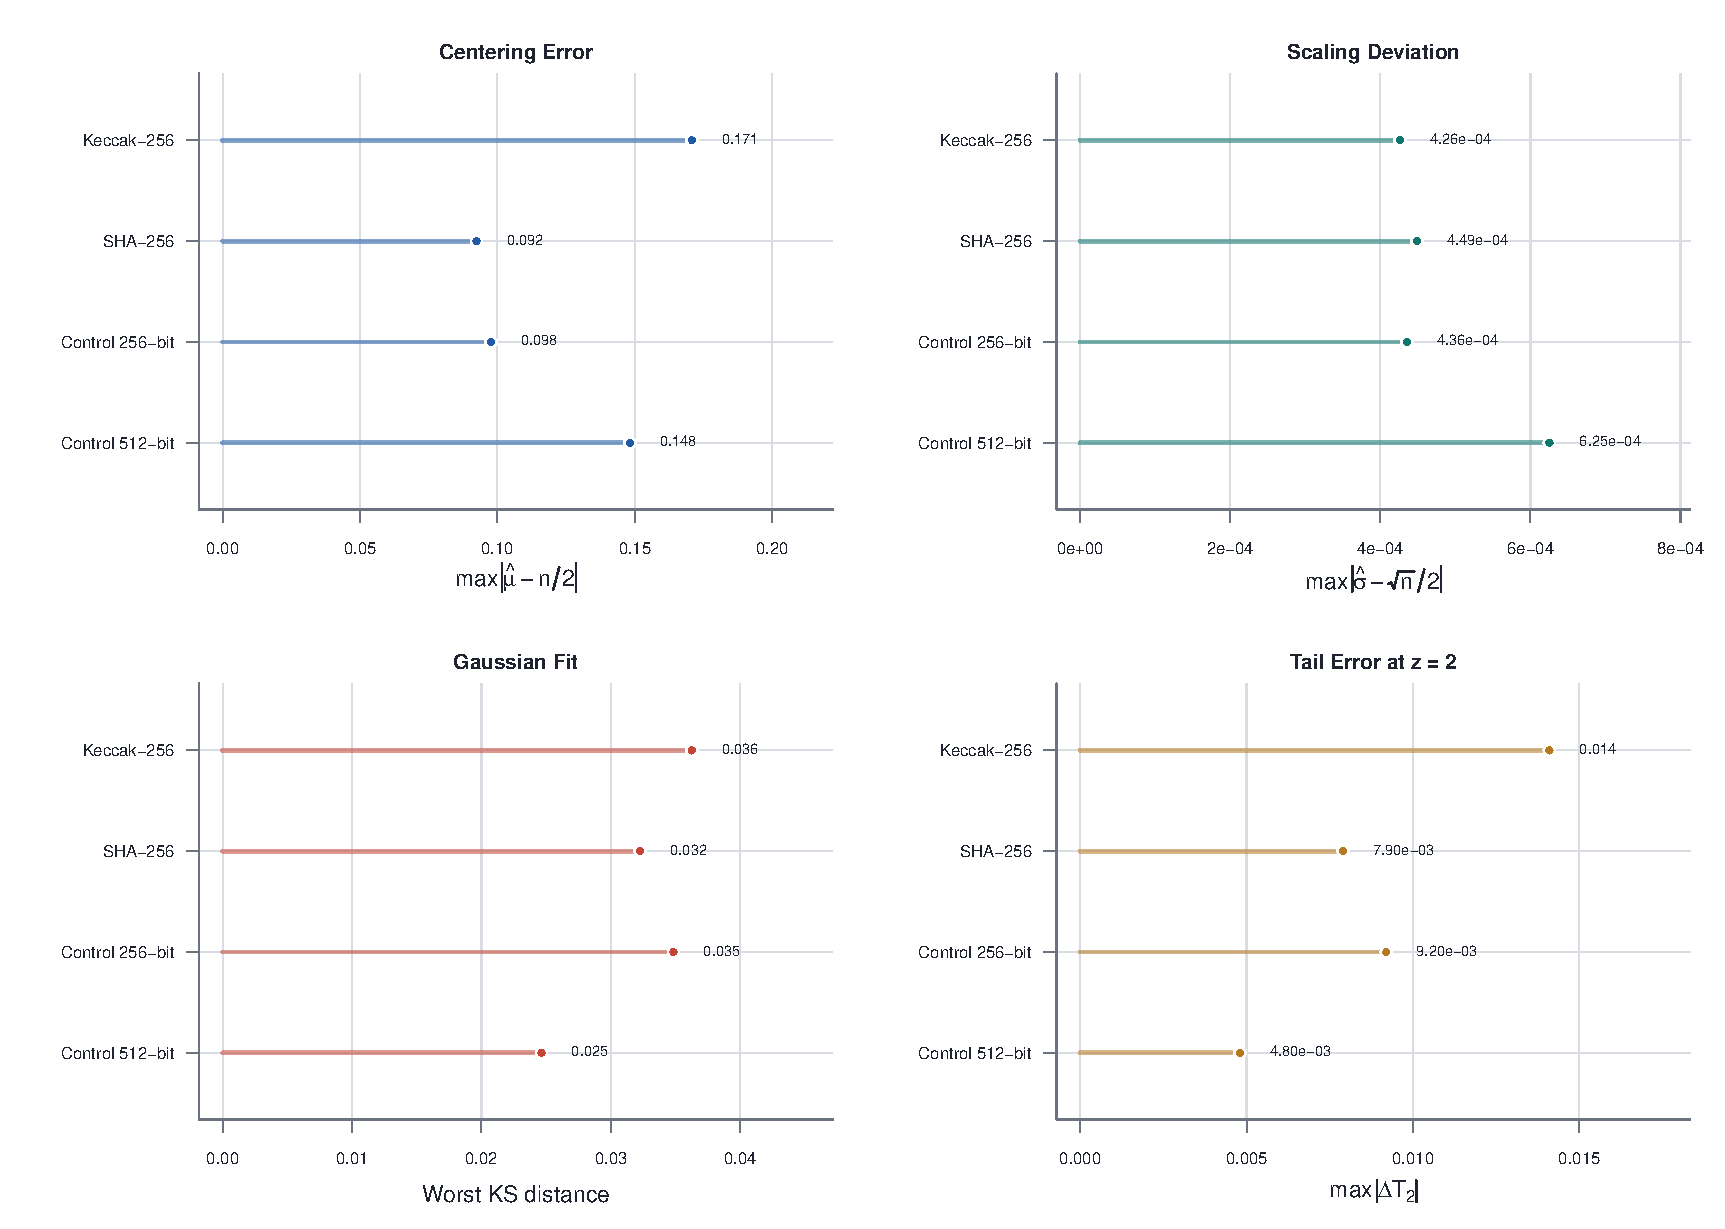
\includegraphics[width=\textwidth]{figures/cross_vm_overview_pub.pdf}
\caption{Cross-VM summary of worst normalization and Gaussian-fit diagnostics
across the tested primitives and widths.}
\label{fig:cross-vm-overview}
\end{figure}

\begin{table}[htbp]
\centering
\small
\begin{tabular}{lrrrrrr}
\hline
Primitive & $n$ & $|\Delta\mu|$ & $|\Delta\sigma|$ & KS & $|\Delta T_2|$ & Max $|\rho_h|$ \\
\hline
Keccak-256 & 256 & 0.1708 & 0.0004 & 0.0363 & 0.0141 & 0.0354 \\
SHA-256 & 256 & 0.0924 & 0.0004 & 0.0323 & 0.0079 & 0.0286 \\
Fair-bit control (256-bit) & 256 & 0.0977 & 0.0004 & 0.0348 & 0.0092 & 0.0253 \\
Fair-bit control (512-bit) & 512 & 0.1482 & 0.0006 & 0.0246 & 0.0048 & 0.0218 \\
\hline
\end{tabular}

\caption{Summary diagnostics for the expanded multi-VM study. The sequence
column reports the largest absolute autocorrelation observed in repeated-output
chains up to lag $30$.}
\label{tab:cross-vm-summary}
\end{table}

Figure~\ref{fig:cross-vm-dependence} shows that the corresponding dependence
diagnostics tell the same story. The worst bit-level autocorrelation up to
lag $30$ is $0.044$ for Keccak-256, $0.052$ for SHA-256, and $0.041$ and
$0.045$ for the two controls; the SHA-256 value is the largest single
dependence statistic in the study, and it exceeds the control by less than the
spread between the two controls themselves. The worst repeated-sequence
lag-1 correlation is $0.018$ for Keccak-256, $0.023$ for SHA-256, and $0.017$
for the 256-bit control, and the worst sequence autocorrelation up to lag
$30$ is $0.035$, $0.029$, and $0.025$. In the 512-bit control the worst lag-1
correlation is $0.008$ and the worst sequence autocorrelation is $0.022$.

\begin{figure}[htbp]
\centering
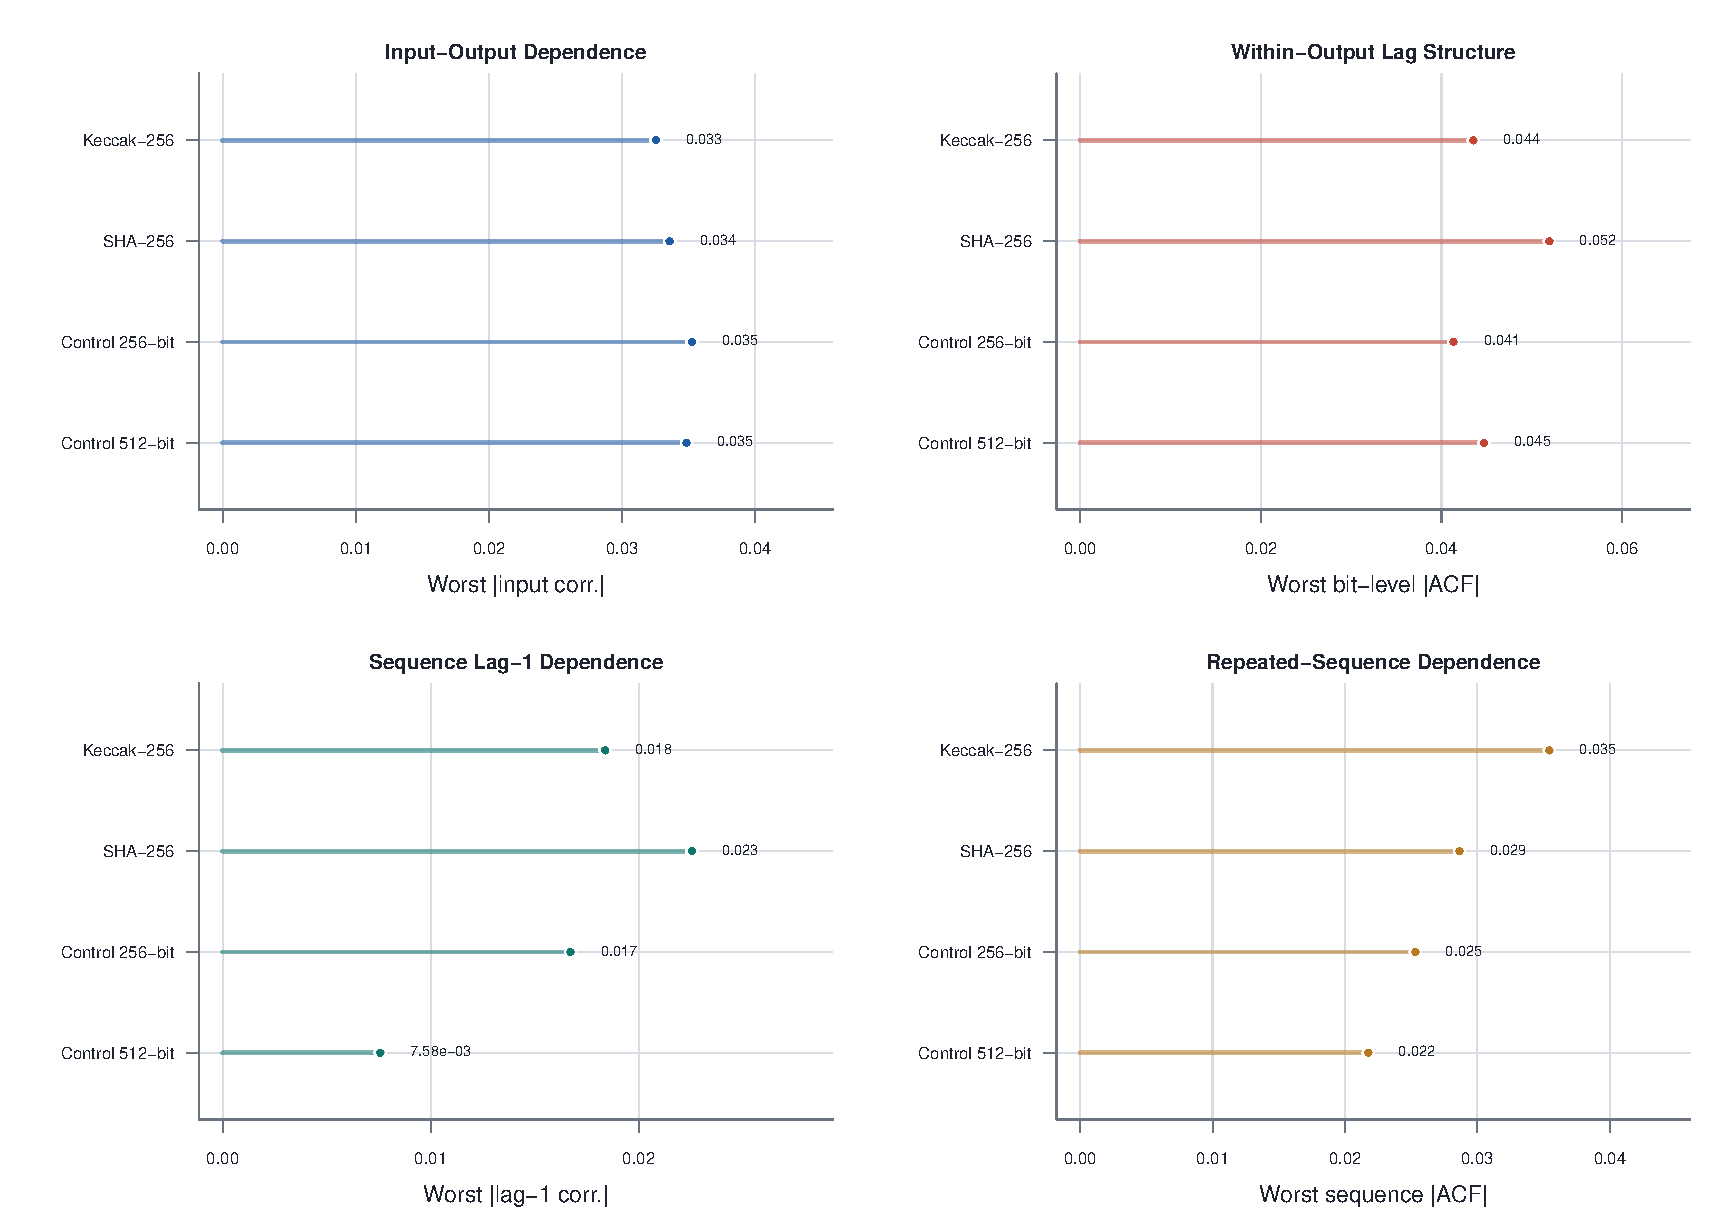
\includegraphics[width=\textwidth]{figures/cross_vm_dependence_pub.pdf}
\caption{Cross-VM summary of input-output, within-output, and repeated-sequence
dependence diagnostics.}
\label{fig:cross-vm-dependence}
\end{figure}

The pairwise similarity measures remain highly stable across the tested targets.
Table~\ref{tab:cross-vm-pairwise} shows that the mean Rogers-Tanimoto
similarity equals its fair-coin value $1/3$ and the mean Sokal-Michener
similarity equals its fair-coin value $1/2$ to four decimals for every target,
and that the largest observed absolute phi-correlation is $0.041$ for
Keccak-256, $0.046$ for SHA-256, and $0.041$ and $0.044$ for the controls. The
two similarity indices are monotone transforms of the same match count and are
reported for comparability with the classical fair-coin baselines; the
phi-correlation carries the pairwise information, and on that statistic the
hash primitives again fall within the range spanned by the controls.

\begin{table}[htbp]
\centering
\small
\begin{tabular}{lrrrr}
\hline
Primitive & Mean RT & Mean SM & Mean $|\phi|$ & Max $|\phi|$ \\
\hline
Keccak-256 & 0.3333 & 0.5000 & 0.0080 & 0.0408 \\
SHA-256 & 0.3333 & 0.5000 & 0.0079 & 0.0461 \\
Fair-bit control (256-bit) & 0.3333 & 0.5000 & 0.0079 & 0.0410 \\
Fair-bit control (512-bit) & 0.3333 & 0.5000 & 0.0079 & 0.0441 \\
\hline
\end{tabular}

\caption{Pairwise binary-sequence similarity and correlation diagnostics for the
baseline sequential family in the expanded multi-VM study.}
\label{tab:cross-vm-pairwise}
\end{table}

\section{Uniformity and Dependence Diagnostics}

Figure~\ref{fig:uniformity} shows the empirical mean of each bit with
Bonferroni-adjusted bands. Across all six input families, the bit-wise
probabilities remain close to $0.5$ and do not show an obvious positional
pattern. In the current run, the largest observed absolute deviation
$|\hat p_i - 0.5|$ lies between roughly $0.014$ and $0.019$ across the six
families. Exactly one of the $6\times256 = 1{,}536$ bit means falls outside
its band: bit $\hat p_i = 0.5192$ in Experiment~1.1, at $z = 3.84$ against a
per-family Bonferroni threshold of $z = 3.73$. Each family has a $5\%$ chance
of producing at least one such exceedance under the null, so one exceedance
among six families is unremarkable, and the corresponding maximum for the
fair-bit control in the expanded study, $0.018$, is of the same size.

\begin{figure}[htbp]
\centering
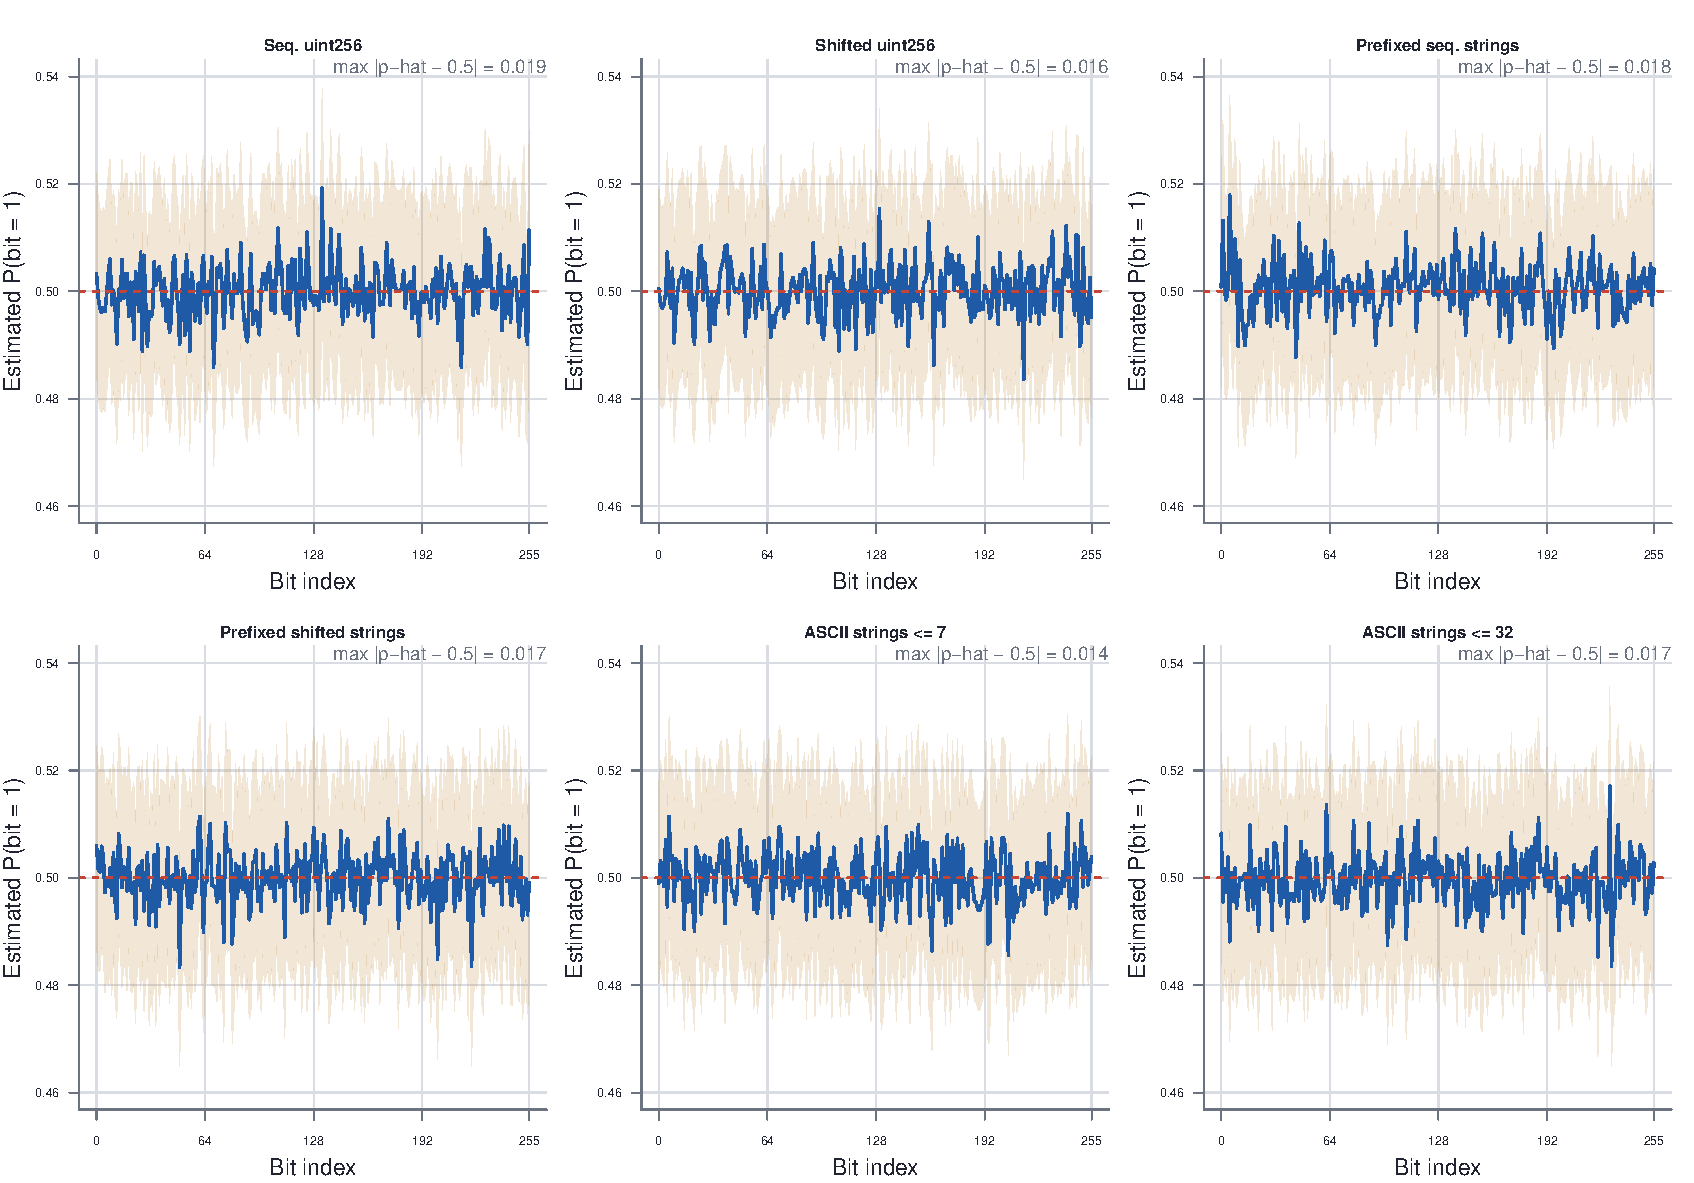
\includegraphics[width=\textwidth]{figures/uniformity_panels_pub.pdf}
\caption{Bit-wise empirical means with Bonferroni-adjusted bands for the six
one-shot input families.}
\label{fig:uniformity}
\end{figure}

Figure~\ref{fig:pairwise} shows pairwise similarity and phi-correlation
diagnostics for all $\binom{256}{2}$ bit pairs in the baseline sequential
integer experiment. The phi-correlation distribution is centered near zero, and
the similarity measures stay close to their fair-coin baselines. This is useful
evidence against simple pairwise dependence, though not a proof that higher
order dependence is absent.

\begin{figure}[htbp]
\centering
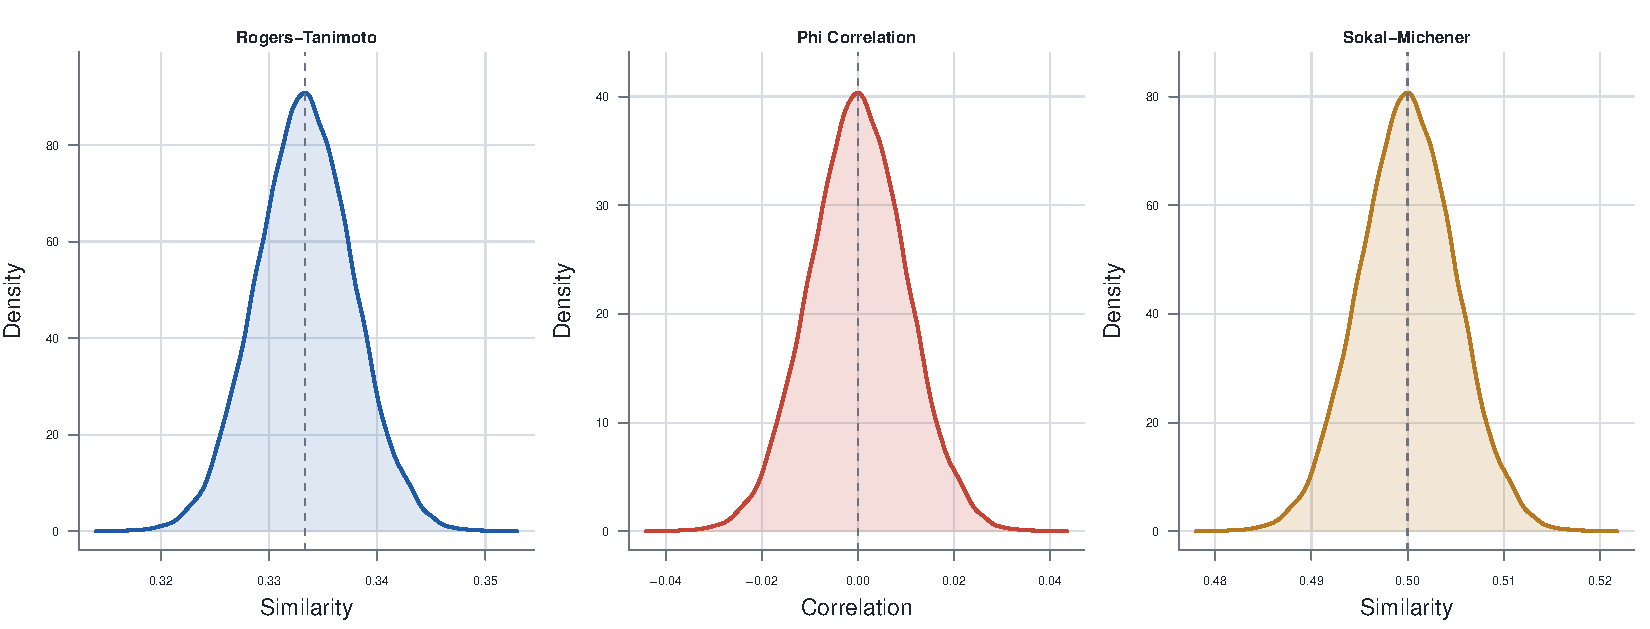
\includegraphics[width=\textwidth]{figures/pairwise_metrics_pub.pdf}
\caption{Pairwise similarity and correlation diagnostics for the baseline
sequential integer experiment.}
\label{fig:pairwise}
\end{figure}

The next dependence check groups each 256-bit digest into 16 non-overlapping
16-bit blocks and computes the Hamming weight of each block. If higher-order
structure were present in a way that directly affects the popcount statistic,
one possible symptom would be correlation among these block-level weights.
Table~\ref{tab:block-popcount} reports the mean and maximum absolute
correlation across the $\binom{16}{2}$ block pairs for each one-shot family.
The mean absolute block correlation remains below about $0.009$, and the
largest observed absolute block correlation is about $0.033$. This does not
prove block independence, but it adds a statistic-level dependence check beyond
individual bit pairs.

\begin{table}[htbp]
\centering
\small
\begin{tabular}{lrr}
\hline
Experiment & Mean block $|r|$ & Max block $|r|$ \\
\hline
Experiment 1.1 & 0.0072 & 0.0263 \\
Experiment 1.2 & 0.0082 & 0.0302 \\
Experiment 2.1 & 0.0069 & 0.0309 \\
Experiment 2.2 & 0.0073 & 0.0325 \\
Experiment 3.1 & 0.0083 & 0.0268 \\
Experiment 3.2 & 0.0074 & 0.0283 \\
\hline
\end{tabular}

\caption{Correlation diagnostics for Hamming weights of 16 non-overlapping
16-bit blocks within each 256-bit output.}
\label{tab:block-popcount}
\end{table}

Figure~\ref{fig:input-corr} studies whether simple input order survives hashing
in the sequential families. The observed input-bit correlations fluctuate
tightly around zero with no persistent structure by bit position. In this run,
the largest absolute input-bit correlation is about $0.033$.

\begin{figure}[htbp]
\centering
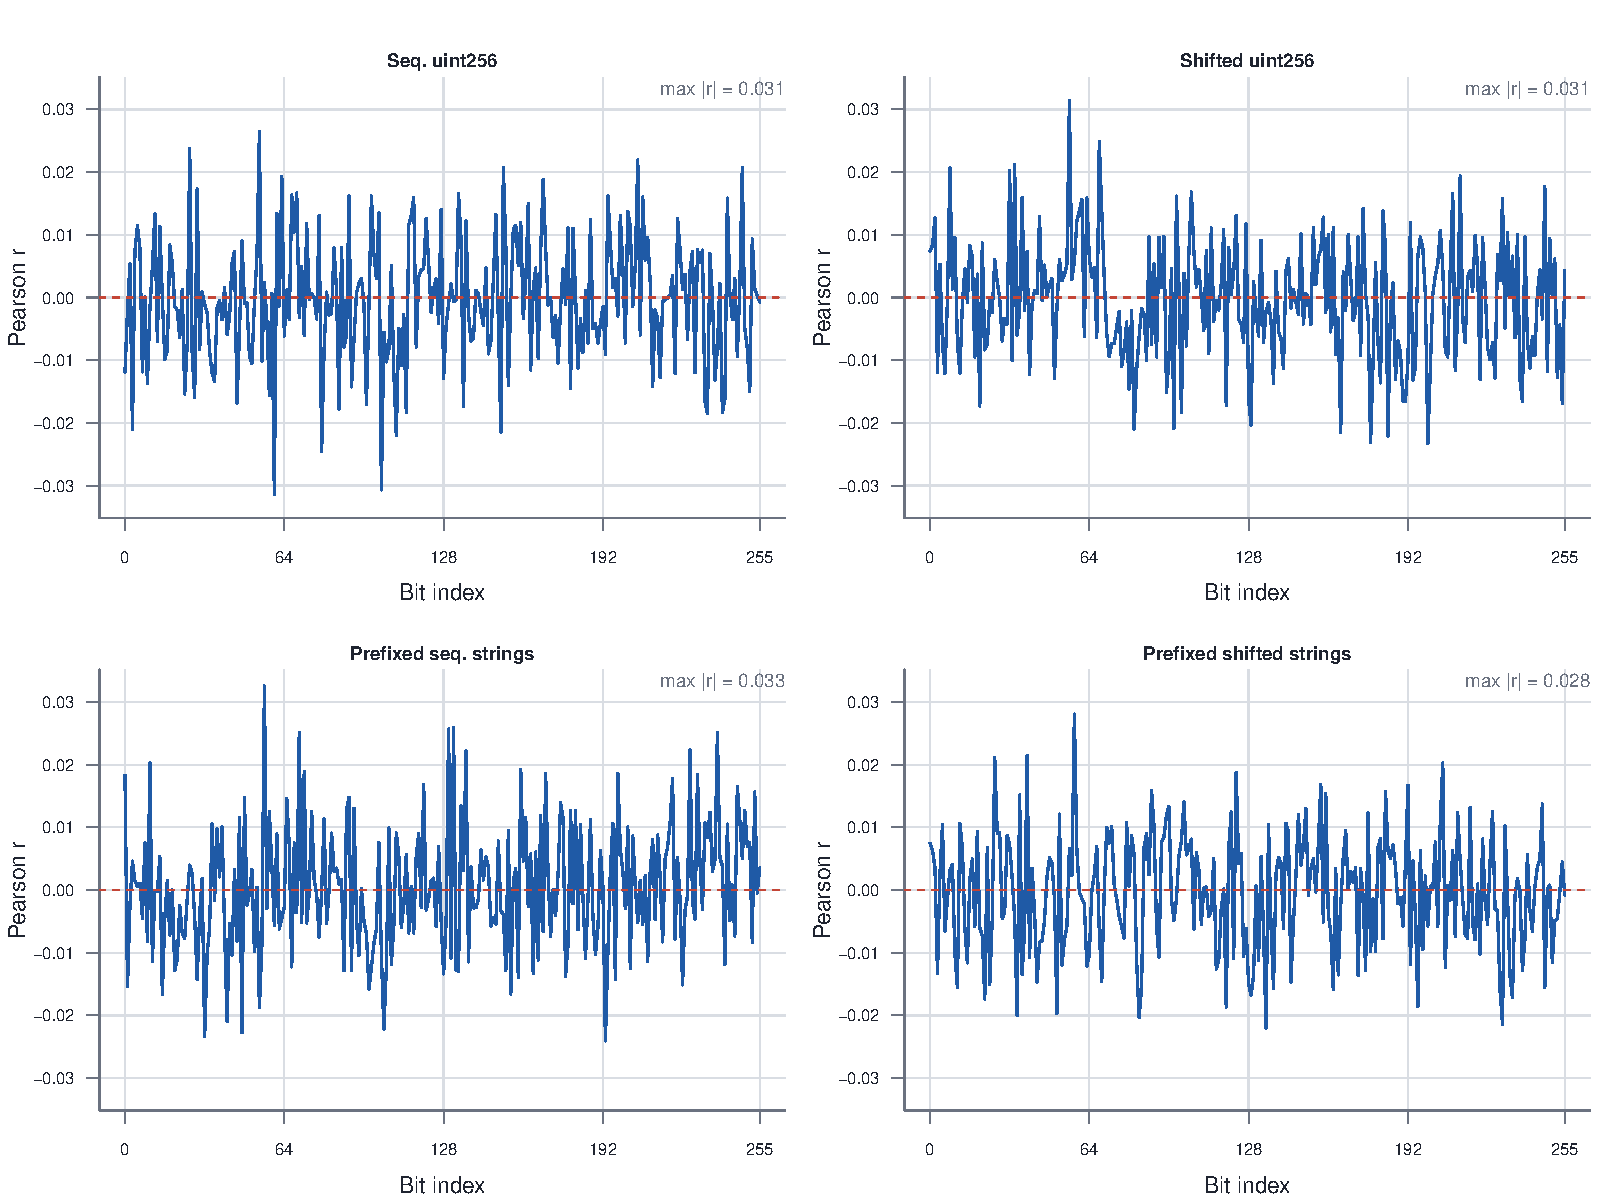
\includegraphics[width=0.92\textwidth]{figures/input_correlation_panels_pub.pdf}
\caption{Pearson correlation between input index and each output bit for the
sequential input families.}
\label{fig:input-corr}
\end{figure}

Figure~\ref{fig:bit-acf} summarizes bit-level autocorrelation for lags $1$
through $30$ in the sequential experiments. The largest observed maximum
absolute autocorrelation in the current run is below $0.044$, again suggesting
that simple short-lag structure is weak in the tested regimes.

\begin{figure}[htbp]
\centering
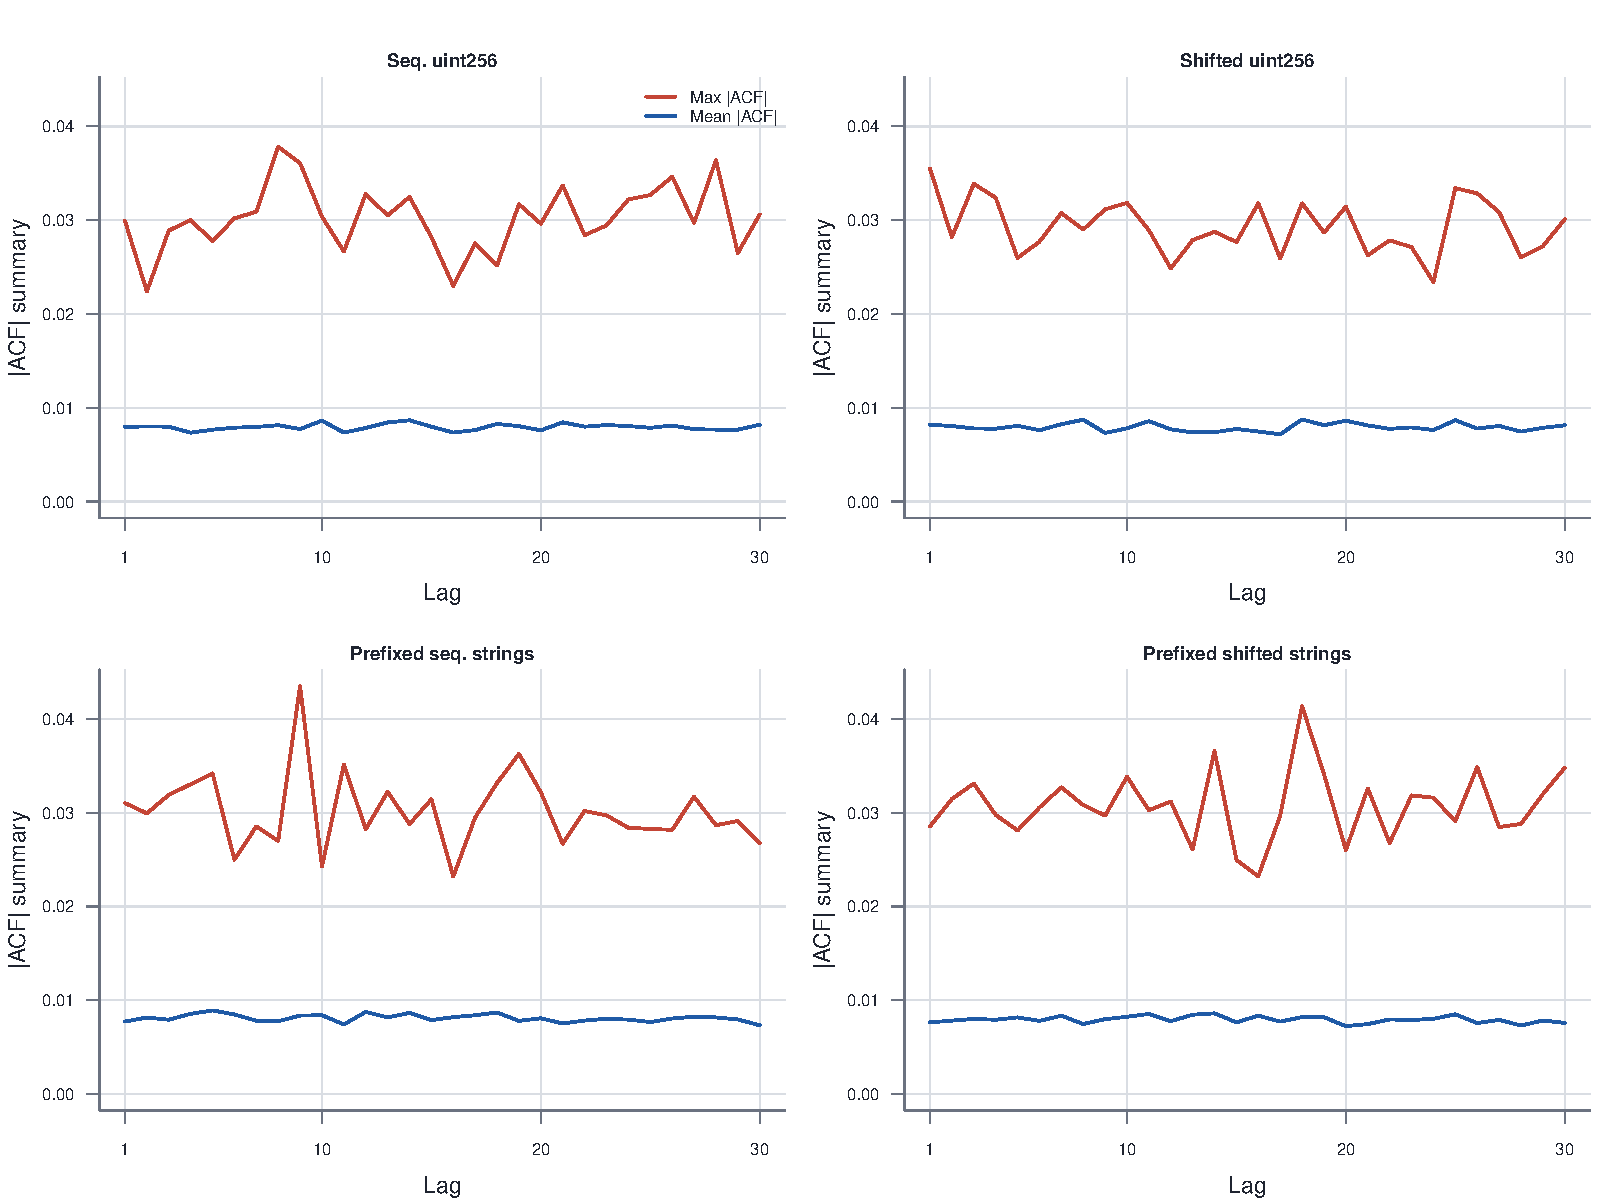
\includegraphics[width=0.92\textwidth]{figures/autocorrelation_panels_pub.pdf}
\caption{Mean and maximum absolute bit-level autocorrelation by lag for the
sequential input families.}
\label{fig:bit-acf}
\end{figure}

\section{Normalization and Gaussian-Fit Diagnostics}

The practical Solidity normalization is based on the fixed constants $128$ and
$8$. By the corollary of Section~\ref{sec:lyapunov}, the quality of that normalization is
governed by the summed bit bias $B_n = \hat\mu - 128$, where
\[
\hat\mu = \sum_{i=1}^{256} \hat p_i,
\qquad
\hat\sigma = \sqrt{\sum_{i=1}^{256} \hat p_i(1-\hat p_i)}
\]
are the centering and scaling implied by the estimated marginals.
Figure~\ref{fig:normalization} and Table~\ref{tab:normalization} report both,
together with the standardized centering shift $(\hat\mu-128)/8$. In the
present run the largest $|\hat\mu-128|$ is $0.171$ (Experiment~2.1), which
shifts the standardized output by $0.021$ standard deviations; the other five
families shift it by at most $0.014$. The standard error of $\hat\mu$ at
$10{,}000$ draws is $8/\sqrt{10{,}000}=0.08$, so the Experiment~2.1 value is
a $2.1$-standard-error fluctuation rather than a systematic offset; the
$10^{6}$-draw study of Section~\ref{sec:tails} confirms this, with
$|\hat\mu-128|\le 0.011$ across all ten targets, a centering shift of at most
$0.0014$ standard deviations.

The implied scale $\hat\sigma$ equals $7.9996$ in every family. That agreement
is not evidence: as the corollary shows, it is forced by the smallness of the
individual biases, and $\hat\sigma$ is computed under the independence
assumption it might be hoped to test. The informative quantity is instead the
ratio of the observed popcount variance $s_S^2$ to the independence-implied
variance $\hat\sigma^2$, which equals $1$ under independent bits and moves
away from $1$ if the bits are positively or negatively associated in a way
that affects the sum. Table~\ref{tab:normalization} reports this ratio; it
lies between $0.988$ and $1.017$ across the six families. With $10{,}000$
near-Gaussian samples the sampling standard deviation of a variance ratio is
about $\sqrt{2/10{,}000}\approx 0.014$, so every observed ratio is within
$1.2$ standard errors of $1$. This is a dependence check at the level of the
statistic the sampler actually consumes, and it is the strongest evidence in
the paper that the independence assumption behind the Poisson-binomial model
is adequate for the Hamming weight.

\begin{figure}[htbp]
\centering
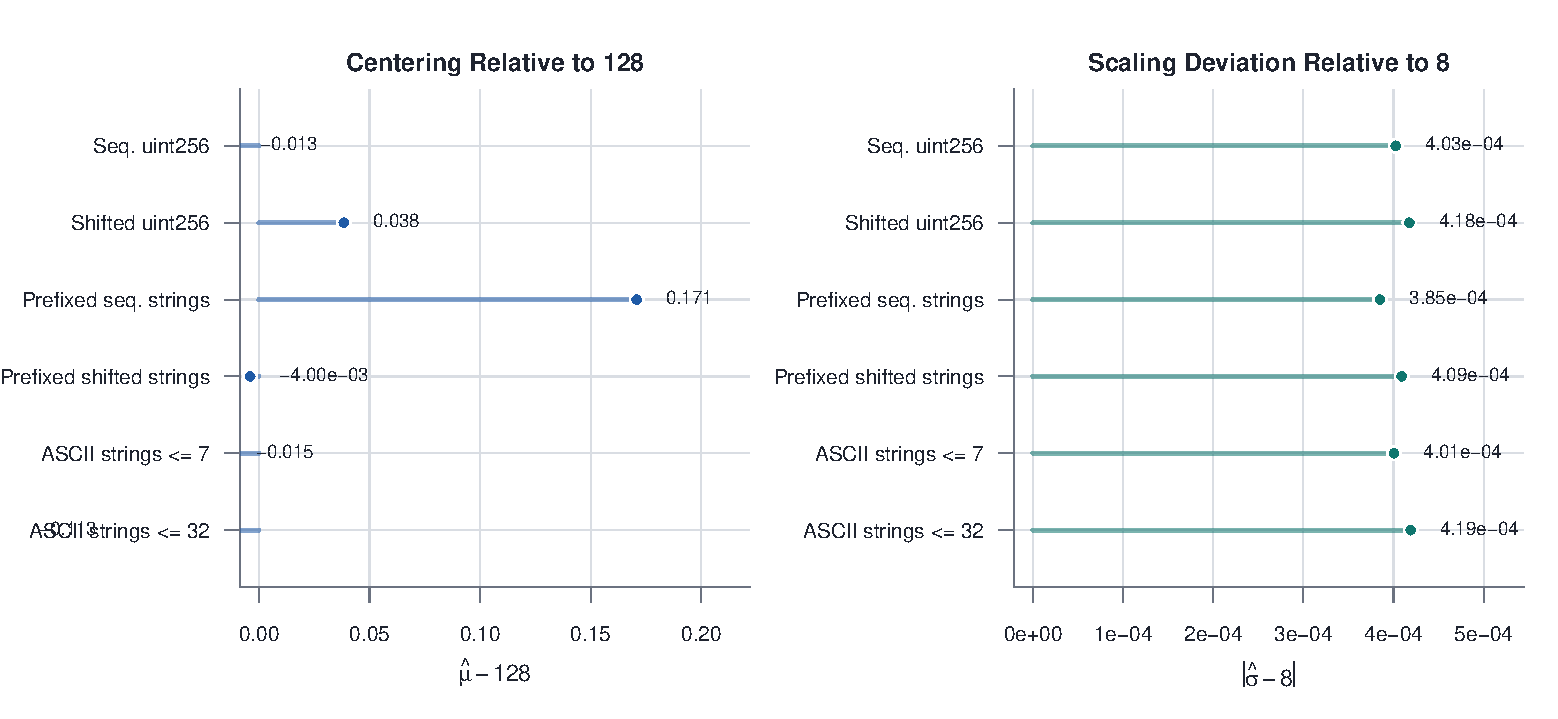
\includegraphics[width=0.92\textwidth]{figures/normalization_errors_pub.pdf}
\caption{Empirical deviations of $(\hat\mu, \hat\sigma)$ from the practical
constants $(128, 8)$.}
\label{fig:normalization}
\end{figure}

\begin{table}[htbp]
\centering
\small
\begin{tabular}{lrrrrrr}
\hline
Experiment & $\hat\mu$ & $\hat\mu-128$ & $(\hat\mu-128)/8$ & $\hat\sigma$ & $s_S$ & $s_S^2/\hat\sigma^2$ \\
\hline
Experiment 1.1 & 127.9873 & -0.0127 & -0.0016 & 7.9996 & 7.9854 & 0.9964 \\
Experiment 1.2 & 128.0384 & 0.0384 & 0.0048 & 7.9996 & 7.9520 & 0.9881 \\
Experiment 2.1 & 128.1708 & 0.1708 & 0.0213 & 7.9996 & 8.0663 & 1.0167 \\
Experiment 2.2 & 127.9960 & -0.0040 & -0.0005 & 7.9996 & 8.0182 & 1.0047 \\
Experiment 3.1 & 127.9854 & -0.0146 & -0.0018 & 7.9996 & 7.9888 & 0.9973 \\
Experiment 3.2 & 127.8874 & -0.1126 & -0.0141 & 7.9996 & 7.9731 & 0.9934 \\
\hline
\end{tabular}

\caption{Centering and scaling diagnostics for the six one-shot families.
$\hat\mu$ and $\hat\sigma$ are the mean and standard deviation implied by the
estimated bit probabilities under independence, $(\hat\mu-128)/8$ is the
resulting shift of the standardized output, $s_S$ is the observed standard
deviation of the popcount, and $s_S^2/\hat\sigma^2$ is the variance ratio,
which equals $1$ under independent bits.}
\label{tab:normalization}
\end{table}

Figure~\ref{fig:cdf} compares the empirical popcount CDF to the Gaussian CDF
with mean $128$ and standard deviation $8$. The fit is already visually close.
Figures~\ref{fig:qq} and \ref{fig:tails} extend that comparison with QQ plots
and two-sided tail probabilities for all six one-shot input families.

\begin{figure}[htbp]
\centering
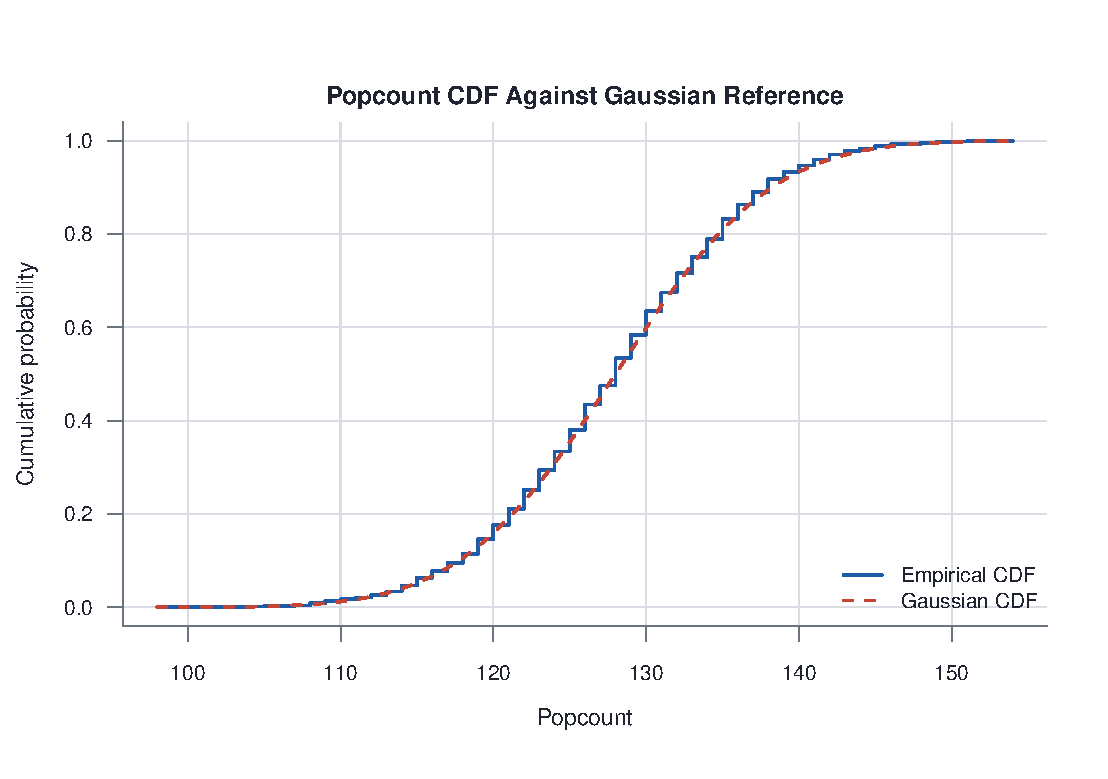
\includegraphics[width=0.78\textwidth]{figures/popcount_cdf_pub.pdf}
\caption{Empirical CDF of the popcount against the Gaussian CDF with mean $128$
and standard deviation $8$.}
\label{fig:cdf}
\end{figure}

\begin{figure}[htbp]
\centering
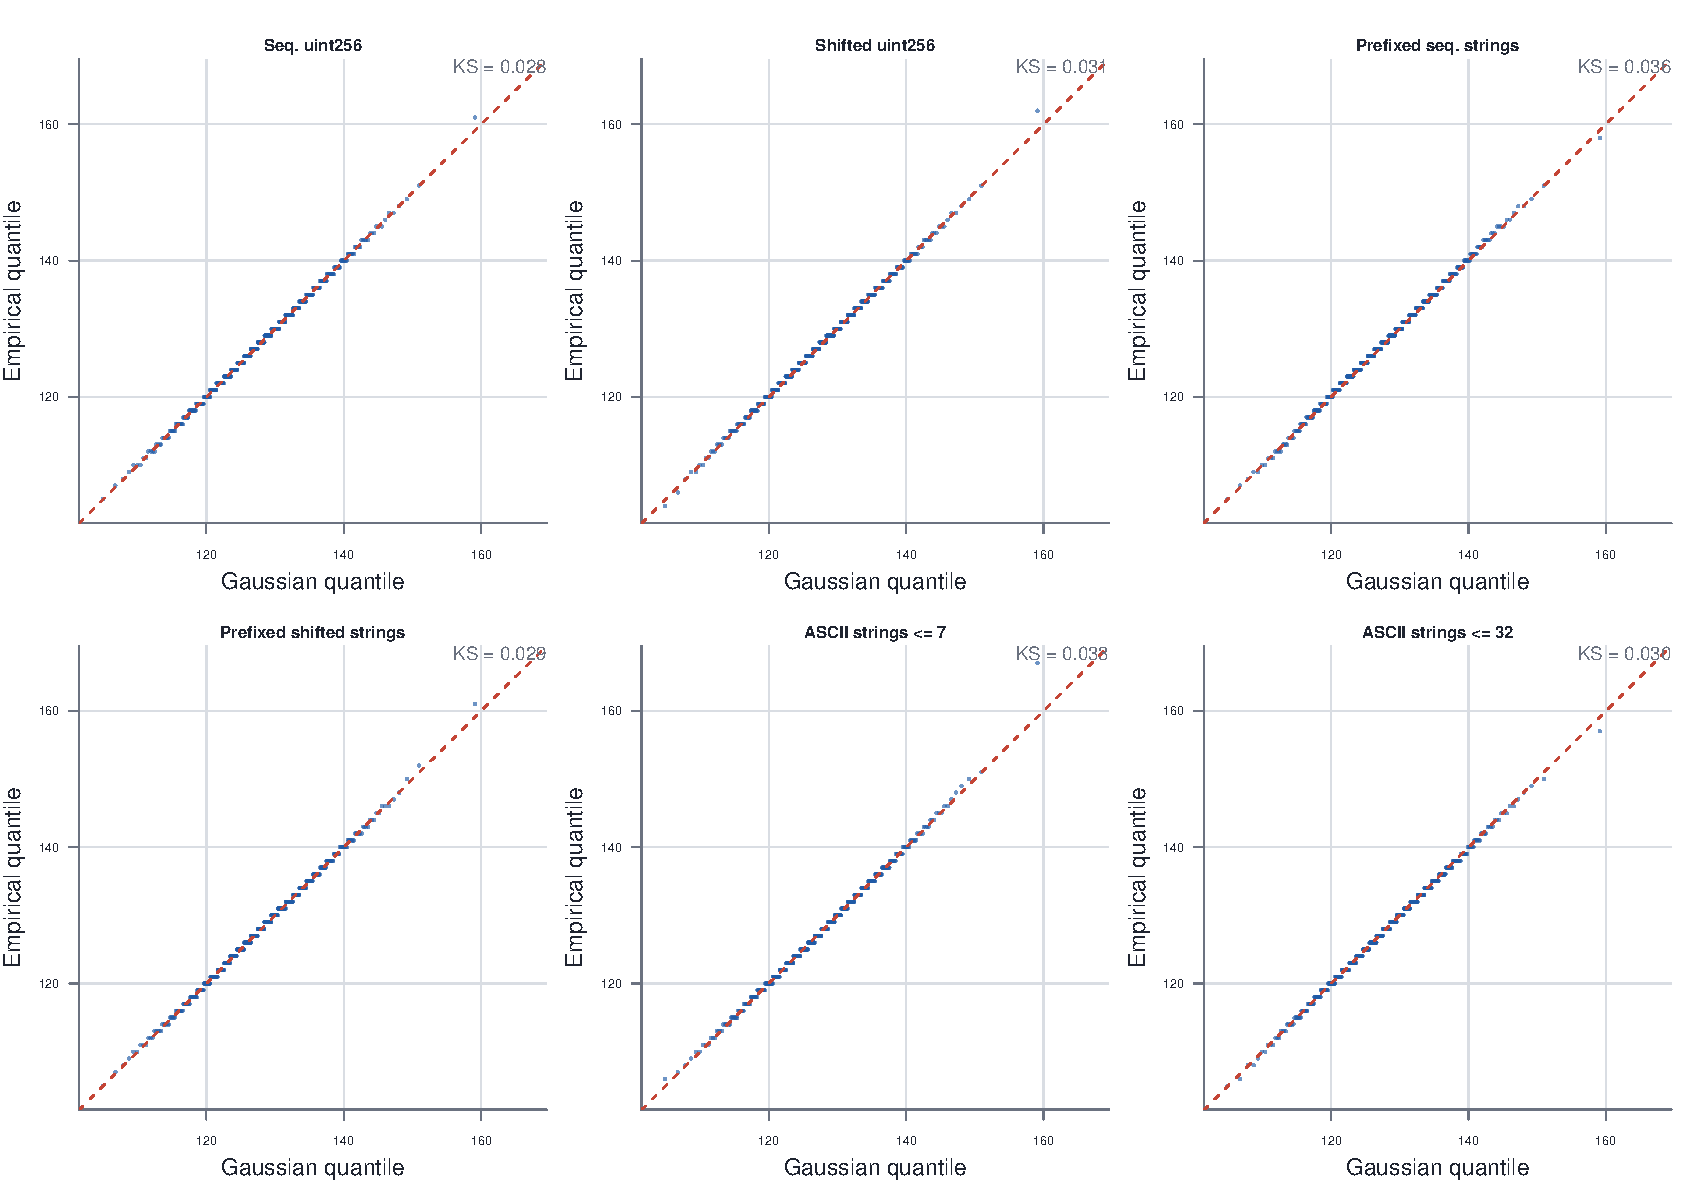
\includegraphics[width=\textwidth]{figures/popcount_qq_panels_pub.pdf}
\caption{QQ diagnostics comparing empirical popcount quantiles to the quantiles
of $N(128,8^2)$.}
\label{fig:qq}
\end{figure}

\begin{figure}[htbp]
\centering
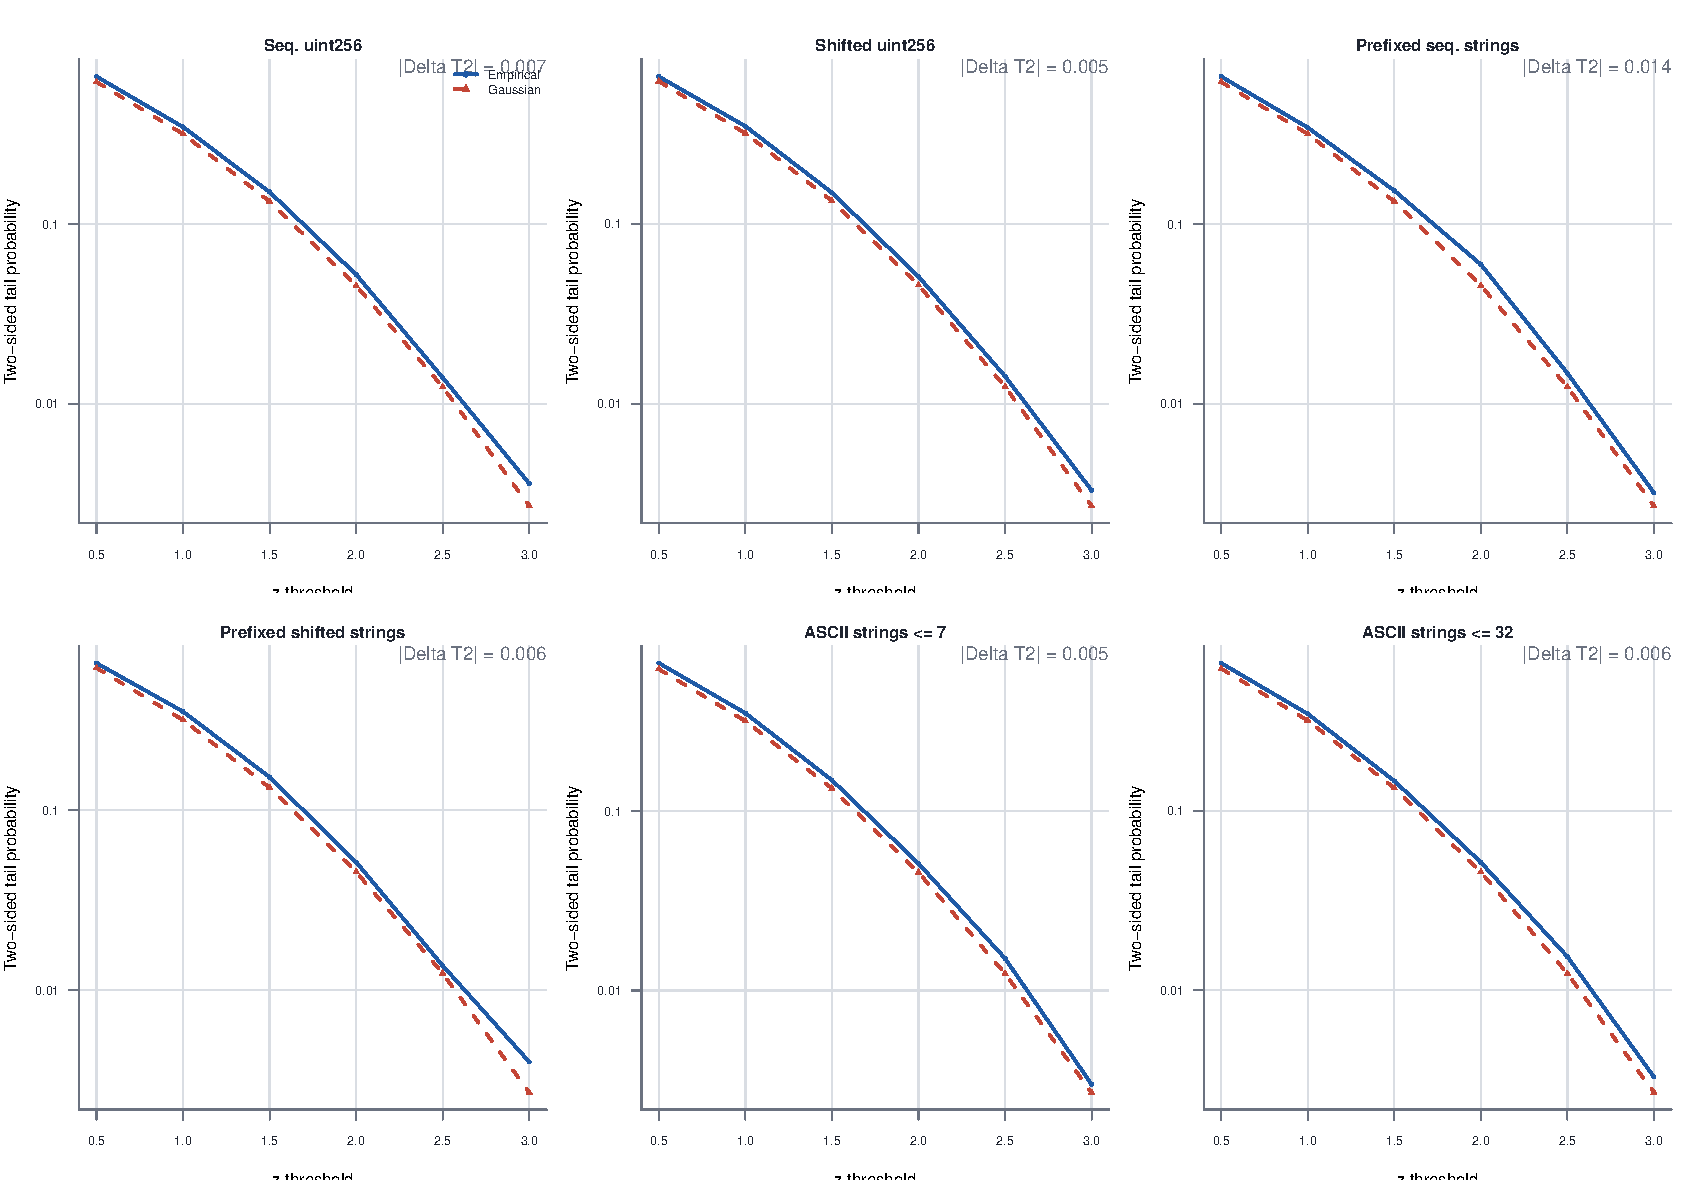
\includegraphics[width=\textwidth]{figures/popcount_tail_panels_pub.pdf}
\caption{Empirical and Gaussian two-sided tail probabilities for the
standardized popcount.}
\label{fig:tails}
\end{figure}

Table~\ref{tab:distribution} summarizes the fit using the Kolmogorov-Smirnov
and Wasserstein-1 distances to two references, the continuous
$\mathcal{N}(128,8^2)$ benchmark and the exact $\mathrm{Binomial}(256,\tfrac12)$
law, together with skewness, excess kurtosis, and the absolute two-sided tail
error at $z=2$. Against the continuous normal, the Kolmogorov-Smirnov distance
lies between $0.028$ and $0.036$ and the Wasserstein distance between $0.25$
and $0.29$; the absolute tail error at $z=2$ lies between $0.005$ and $0.014$.

Those continuous-reference distances are dominated by the lattice, not by the
bits. The popcount takes integer values, so its CDF is a step function, and
the Kolmogorov-Smirnov distance between the \emph{exact}
$\mathrm{Binomial}(256,\tfrac12)$ law and $\mathcal{N}(128,8^2)$, computed with
the same two-sided convention, is already $0.0249$; similarly, rounding a
continuous variable to a unit lattice contributes about $0.25$ to the
Wasserstein distance. Once the reference is the exact binomial law, the
Kolmogorov-Smirnov distance drops to between $0.004$ and $0.012$ and the
Wasserstein distance to between $0.05$ and $0.19$. For comparison, the usual
$5\%$ critical value at $10{,}000$ samples is $1.36/\sqrt{10000}=0.0136$, so
none of the six families rejects the exact fair-coin binomial law at that
level, whereas all six would reject a continuous normal null, as any lattice
variable must. The right reading of Table~\ref{tab:distribution} is therefore
that the Hamming weight of \texttt{keccak256} is compatible with the Hamming
weight of fair independent bits, and that the residual distance to a
continuous Gaussian is the discretization the on-chain application has
already accepted.

\begin{table}[htbp]
\centering
\small
\begin{tabular}{lrrrrrrr}
\hline
Experiment & KS$_{\mathcal N}$ & KS$_{\mathrm{Bin}}$ & $W_1^{\mathcal N}$ & $W_1^{\mathrm{Bin}}$ & Skewness & Excess Kurtosis & $|\Delta T_2|$ \\
\hline
Experiment 1.1 & 0.0282 & 0.0036 & 0.2546 & 0.0490 & 0.0007 & -0.0153 & 0.0069 \\
Experiment 1.2 & 0.0311 & 0.0062 & 0.2624 & 0.0838 & -0.0273 & 0.0419 & 0.0053 \\
Experiment 2.1 & 0.0363 & 0.0117 & 0.2924 & 0.1927 & -0.0137 & 0.0437 & 0.0141 \\
Experiment 2.2 & 0.0288 & 0.0052 & 0.2591 & 0.0669 & 0.0019 & 0.0175 & 0.0060 \\
Experiment 3.1 & 0.0329 & 0.0090 & 0.2684 & 0.0972 & 0.0602 & 0.0009 & 0.0055 \\
Experiment 3.2 & 0.0302 & 0.0067 & 0.2695 & 0.1129 & -0.0235 & 0.0000 & 0.0061 \\
\hline
\end{tabular}

\caption{Finite-sample distributional diagnostics for the popcount.
KS$_{\mathcal N}$ and $W_1^{\mathcal N}$ are distances to the continuous
$\mathcal{N}(128,8^2)$ benchmark; KS$_{\mathrm{Bin}}$ and $W_1^{\mathrm{Bin}}$
are distances to the exact $\mathrm{Binomial}(256,\tfrac12)$ law. The
discreteness floor for KS$_{\mathcal N}$ is $0.0249$.}
\label{tab:distribution}
\end{table}

The tail-error column carries the same kind of lattice offset. The two-sided
tail is evaluated at $|S-128|\ge 8z$, and on the lattice that event includes
the atom at exactly $8z$, so the exact binomial tail is systematically
heavier than the uncorrected Gaussian tail: $0.0525$ against $0.0455$ at
$z=2$, a gap of $0.007$ that is present even for perfectly fair independent
bits. Applying the usual continuity correction, that is, comparing with
$2\bigl(1-\Phi((8z-\tfrac12)/8)\bigr)$, reproduces the binomial tail to three
decimals at every $z$ from $1$ to $4$. The observed $|\Delta T_2|$ values of
$0.005$--$0.014$ in Table~\ref{tab:distribution} are therefore mostly this
offset, not a property of the bits.

\subsection{Tails at $10^{6}$ draws}
\label{sec:tails}

With $10{,}000$ draws the two-sided Gaussian tail at $z=3$ corresponds to
about $27$ draws and at $z=4$ to fewer than one, so the diagnostics above say
little about the extreme tails. To address this directly, a separate run
draws $10^{6}$ \texttt{keccak256} popcounts for each of the six one-shot
families and each of the four repeated-hash chains, that is, $10^{7}$ digests
in total, and compares the tails against the exact binomial law.
Table~\ref{tab:tail-1e6} reports the two-sided tail probabilities in units of
$10^{-3}$ at $z=1,\dots,4$, with the Gaussian and binomial references in the
first two rows, and Table~\ref{tab:tail-ks-1e6} the corresponding mean,
standard deviation, and Kolmogorov-Smirnov distance to the binomial law.

\begin{table}[htbp]
\centering
\small
\begin{tabular}{lrrrrrrr}
\hline
Target & $z=1$ & $z=1.5$ & $z=2$ & $z=2.5$ & $z=3$ & $z=3.5$ & $z=4$ \\
\hline
Gaussian & 317.311 & 133.614 & 45.500 & 12.419 & 2.700 & 0.465 & 0.063 \\
Binomial$(256,\tfrac12)$ & 348.521 & 150.435 & 52.472 & 14.628 & 3.231 & 0.561 & 0.076 \\
\hline
Experiment 1.1 & 348.661 & 150.912 & 52.519 & 14.694 & 3.249 & 0.572 & 0.094 \\
Experiment 1.2 & 348.176 & 150.262 & 51.972 & 14.444 & 3.197 & 0.543 & 0.080 \\
Experiment 2.1 & 347.933 & 150.494 & 52.402 & 14.684 & 3.213 & 0.532 & 0.076 \\
Experiment 2.2 & 348.794 & 150.657 & 52.784 & 14.808 & 3.264 & 0.558 & 0.076 \\
Experiment 3.1 & 348.997 & 150.082 & 51.958 & 14.648 & 3.298 & 0.617 & 0.067 \\
Experiment 3.2 & 348.316 & 150.217 & 51.965 & 14.632 & 3.285 & 0.568 & 0.075 \\
Sequence 1 & 347.632 & 150.209 & 51.926 & 14.510 & 3.235 & 0.539 & 0.071 \\
Sequence 2 & 348.127 & 150.600 & 52.666 & 14.691 & 3.278 & 0.548 & 0.086 \\
Sequence 3 & 348.442 & 150.272 & 52.299 & 14.626 & 3.191 & 0.531 & 0.068 \\
Sequence 4 & 348.262 & 149.639 & 52.209 & 14.597 & 3.276 & 0.580 & 0.082 \\
\hline
\end{tabular}

\caption{Two-sided tail probabilities $\mathbb{P}(|S-128|\ge 8z)$ in units of
$10^{-3}$ from $10^{6}$ draws per target, against the continuous Gaussian and
the exact $\mathrm{Binomial}(256,\tfrac12)$ references. At $z=4$ the binomial
reference corresponds to $76$ expected draws.}
\label{tab:tail-1e6}
\end{table}

\begin{table}[htbp]
\centering
\small
\begin{tabular}{lrrr}
\hline
Target & Mean & SD & KS$_{\mathrm{Bin}}$ \\
\hline
Experiment 1.1 & 128.0048 & 8.0019 & 0.00081 \\
Experiment 1.2 & 128.0051 & 7.9904 & 0.00060 \\
Experiment 2.1 & 128.0090 & 7.9967 & 0.00077 \\
Experiment 2.2 & 127.9986 & 8.0078 & 0.00074 \\
Experiment 3.1 & 127.9893 & 7.9950 & 0.00114 \\
Experiment 3.2 & 127.9907 & 7.9955 & 0.00091 \\
Sequence 1 & 127.9983 & 7.9897 & 0.00059 \\
Sequence 2 & 128.0111 & 8.0015 & 0.00093 \\
Sequence 3 & 127.9995 & 7.9982 & 0.00074 \\
Sequence 4 & 127.9944 & 7.9908 & 0.00067 \\
\hline
\end{tabular}

\caption{Mean, standard deviation, and Kolmogorov-Smirnov distance to the exact
binomial law from $10^{6}$ draws per target. The $5\%$ critical value at this
sample size is $1.36/\sqrt{10^{6}}=0.00136$.}
\label{tab:tail-ks-1e6}
\end{table}

Every target tracks the binomial row, not the Gaussian row, at every
threshold, including $z=4$, where the observed counts range from $67$ to $94$
against $76$ expected. Of the $70$ target-by-threshold comparisons, seven
exceed $1.96$ binomial standard errors in absolute value and the largest is
$2.45$; the thresholds are nested within each target, so these comparisons are
strongly correlated and a modest excess over the nominal $3.5$ is not
surprising, and the deviations show no consistent sign across thresholds. The
Kolmogorov-Smirnov distance to the binomial law lies between $0.0006$ and
$0.0011$ for all ten targets, below the $5\%$ critical value of $0.00136$ at
this sample size, so none of them rejects the fair-coin binomial law even with
a hundred times more data than the main study.

\section{Repeated-Hash Sequence Diagnostics}

The previous sections study isolated hash outputs. The actual generator,
however, is consumed as a sequence. The next question is therefore whether the
recursive map
\[
H_{t+1} = \texttt{keccak256}(H_t)
\]
introduces visible short-lag structure into the popcount sequence
\[
S_t = \text{number of 1's in } H_t.
\]

Figure~\ref{fig:seq-acf} shows the autocorrelation of $S_t$ for four
representative repeated-hash chains and for lags $1$ through $30$.
Figure~\ref{fig:seq-scatter} plots $S_t$ against $S_{t+1}$ for the same chains.
The visual impression is that these chains do not display obvious short-lag
structure. In the current run, the lag-1 correlation lies between roughly
$0.001$ and $0.018$, while the maximum absolute autocorrelation through lag $30$
lies between roughly $0.023$ and $0.035$.

\begin{figure}[htbp]
\centering
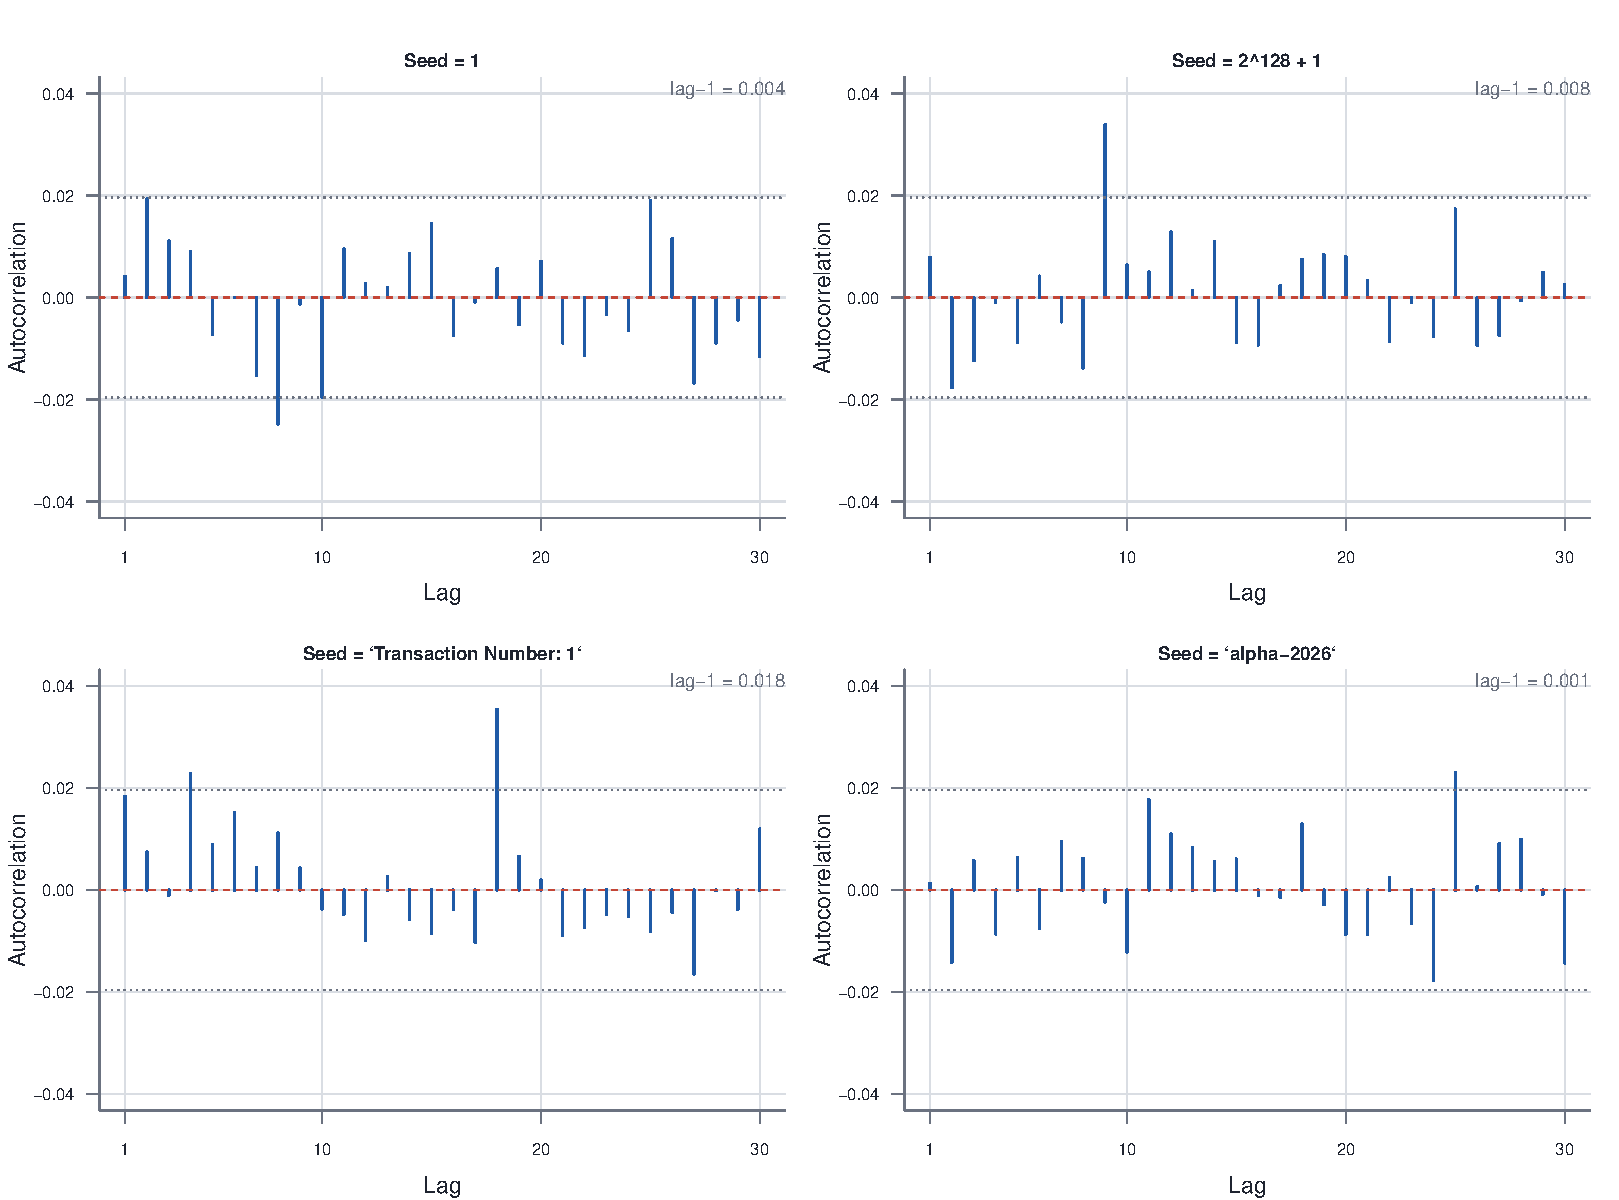
\includegraphics[width=0.92\textwidth]{figures/sequence_acf_panels_pub.pdf}
\caption{Autocorrelation of the popcount sequence for four repeated-hash
chains.}
\label{fig:seq-acf}
\end{figure}

\begin{figure}[htbp]
\centering
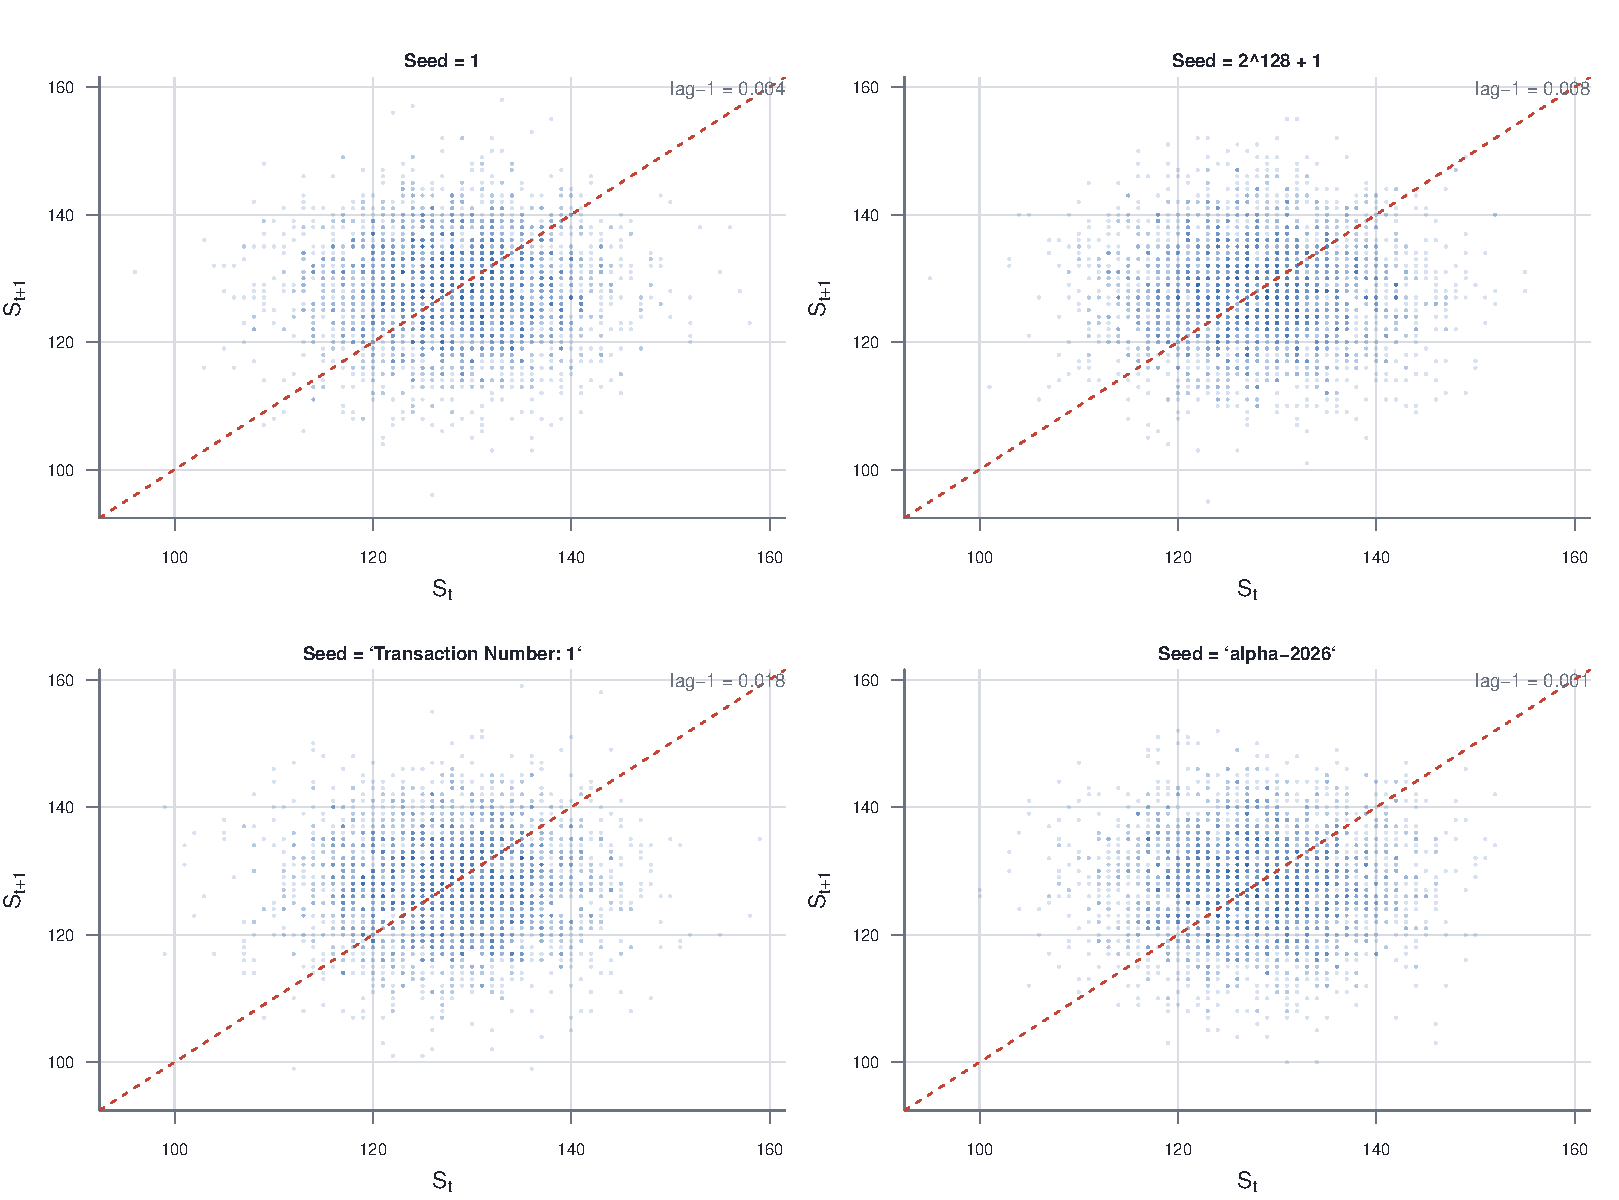
\includegraphics[width=0.92\textwidth]{figures/sequence_scatter_panels_pub.pdf}
\caption{Lag-1 scatter plots for repeated-hash popcount sequences.}
\label{fig:seq-scatter}
\end{figure}

Table~\ref{tab:sequence} summarizes the same study by reporting the mean and
standard deviation of the popcount sequence, the lag-1 correlation, the
largest absolute autocorrelation up to lag $30$, the runs-test $z$-score
about the median $128$, and the absolute two-sided tail error at $z=2$. The
runs-test $z$-scores lie between $-1.50$ and $0.78$, and the tail errors
between $0.003$ and $0.008$, which is again compatible with the absence of
obvious short-lag dependence for the tested seeds.

\begin{table}[htbp]
\centering
\small
\begin{tabular}{lrrrrrr}
\hline
Sequence & Mean Count & SD Count & Lag-1 Corr & Max $|\rho_h|$ & Runs $z$ & $|\Delta T_2|$ \\
\hline
Sequence 1 & 127.9579 & 7.9600 & 0.0042 & 0.0248 & 0.1287 & 0.0027 \\
Sequence 2 & 128.0153 & 7.9580 & 0.0079 & 0.0339 & -0.1537 & 0.0083 \\
Sequence 3 & 128.0109 & 7.9452 & 0.0184 & 0.0354 & -1.4950 & 0.0047 \\
Sequence 4 & 127.8900 & 7.9386 & 0.0013 & 0.0230 & 0.7849 & 0.0068 \\
\hline
\end{tabular}

\caption{Summary diagnostics for repeated-hash popcount sequences.}
\label{tab:sequence}
\end{table}

\section{On-Chain Implications}

The practical interpretation of the numerical study is straightforward. If the
bit probabilities remain close to $0.5$, then the natural centering and scaling
are already close to $(128,8)$. If the popcount distribution is close to a
Gaussian benchmark at $n=256$, then the integer-scaled Solidity output
\[
125S - 16000
\]
is a plausible discrete approximation to a standard normal draw, represented
at integer scale $1000$.

The output is nevertheless a lattice-valued random variable, not a continuous
normal draw, and the integer scale should not be mistaken for resolution. For
$n=256$ and $c=1000$, adjacent possible outputs differ by $125$, because
changing the Hamming weight by one changes $125S-16000$ by $125$; the
effective resolution is therefore $0.125$ standard deviations, not $0.001$,
and the support is confined to $[-16,16]$ standard deviations.
Figure~\ref{fig:integer-output} shows this final integer-scaled distribution
for a representative one-shot family. Doubling the width to $n=512$ improves
the resolution only to $2/\sqrt{512}\approx 0.088$; resolution improves as
$2/\sqrt{n}$, so each additional decimal digit costs a hundredfold increase
in width. This discreteness is usually acceptable for game mechanics,
perturbations, and integer-valued smart-contract logic, but it should be kept
explicit when an application requires a continuous or very fine-grained
distribution.

\begin{figure}[htbp]
\centering
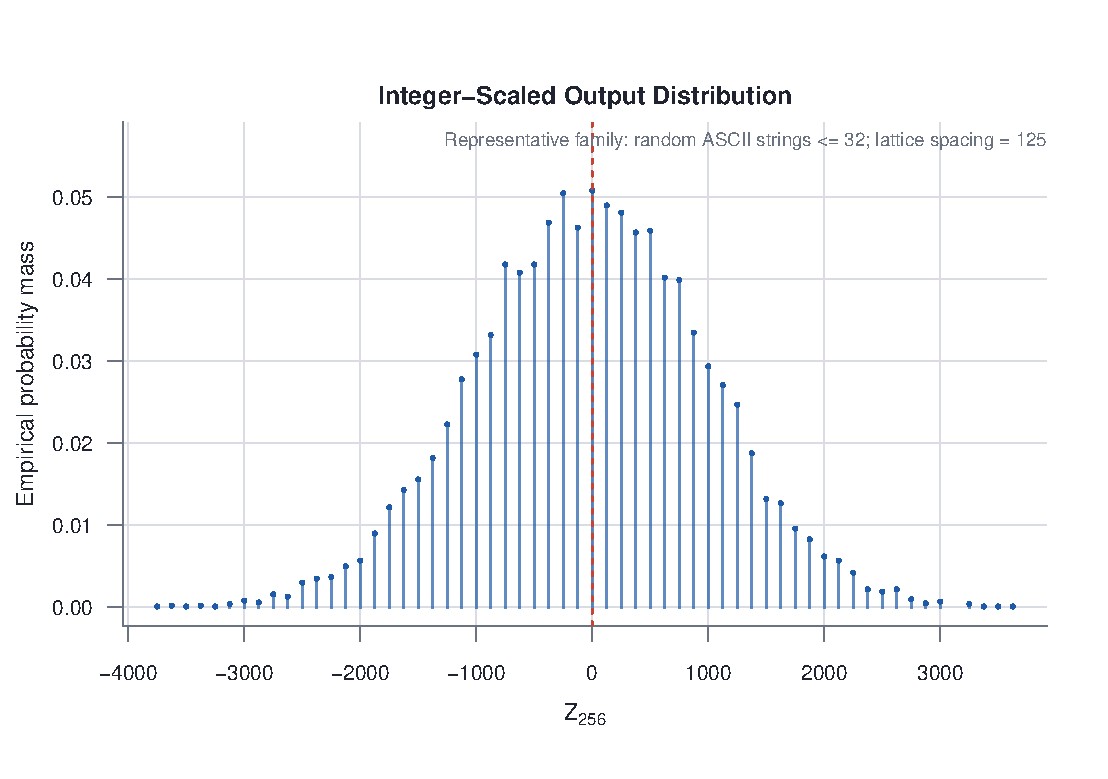
\includegraphics[width=0.78\textwidth]{figures/integer_scaled_output_pub.pdf}
\caption{Empirical distribution of the final integer-scaled output
$Z_{256,1000}=125S-16000$ for the random ASCII input family with length up to
32.}
\label{fig:integer-output}
\end{figure}

This approach is attractive on-chain because it avoids floating-point
operations, trigonometric transforms, and expensive rejection samplers. The
computation reduces to hashing and bit counting. A Box--Muller transform would
require logarithms, square roots, and trigonometric functions, either natively
or through approximations \citep{BoxMuller1958}. Ziggurat or other
rejection-sampling approaches can avoid some transcendental work, but they
introduce tables, branches, and a variable number of iterations
\citep{MarsagliaTsang2000}. The present method has a fixed execution shape
once the entropy input is available, provided the population count itself is
implemented with a fixed instruction count: obtain one VM-native output, count
its bits, and apply a small amount of integer arithmetic.

Table~\ref{tab:gas} reports the measured EVM gas for each stage, obtained with
\texttt{gasleft()} deltas inside a single call over $2{,}000$ chained
\texttt{keccak256} digests (Foundry, \texttt{solc} 0.8.26 with the optimizer
enabled, Cancun EVM). The choice of population-count algorithm matters more
than everything else combined. The textbook Kernighan loop, which clears one
set bit per iteration, averages $7{,}761$ gas and ranges from $6{,}074$ to
$9{,}374$ because its iteration count \emph{is} the Hamming weight; it
therefore also leaks the output value through gas consumption. A SWAR
(SIMD-within-a-register) reduction computes the same count in $233$ gas with
no data dependence. With the SWAR count, one Gaussian draw costs about $530$
gas in total, roughly $2.5\%$ of the $21{,}000$ base cost of a transaction,
and about $15$ times less than the loop-based variant. The price of this
simplicity is that the distributional claim is only as strong as the
probabilistic model and the empirical evidence supporting it.

\begin{table}[htbp]
\centering
\small
\begin{tabular}{lrrrl}
\hline
Stage & Mean gas & Min & Max & Cost shape \\
\hline
\texttt{keccak256} of one 32-byte word & 268 & 221 & 316 & fixed (memory expansion) \\
popcount, Kernighan loop & 7,761 & 6,074 & 9,374 & one iteration per set bit \\
popcount, SWAR reduction & 233 & 233 & 233 & constant \\
integer scaling $125S-16000$ & 29 & 29 & 29 & constant \\
\hline
\end{tabular}
\caption{Measured EVM gas per stage of the $n=256$ transform over $2{,}000$
chained digests. The base transaction cost and calldata are excluded.}
\label{tab:gas}
\end{table}

\begin{table}[htbp]
\centering
\small
\begin{tabular}{lrrrrr}
\hline
Experiment & Max $|\hat p_i-0.5|$ & Mean Count & SD Count & Max $|r|$ & Max $|\rho_h|$ \\
\hline
Experiment 1.1 & 0.0192 & 127.9873 & 7.9854 & 0.0314 & 0.0378 \\
Experiment 1.2 & 0.0164 & 128.0384 & 7.9520 & 0.0314 & 0.0355 \\
Experiment 2.1 & 0.0179 & 128.1708 & 8.0663 & 0.0325 & 0.0435 \\
Experiment 2.2 & 0.0166 & 127.9960 & 8.0182 & 0.0281 & 0.0414 \\
Experiment 3.1 & 0.0144 & 127.9854 & 7.9888 & -- & -- \\
Experiment 3.2 & 0.0171 & 127.8874 & 7.9731 & -- & -- \\
\hline
\end{tabular}

\caption{Summary diagnostics across the six one-shot experiments.}
\label{tab:summary}
\end{table}

\section{Scope and Limitations}

The numerical study provides empirical support for the modeling assumptions, but
it does not prove full joint independence of the output bits of
\texttt{keccak256}, SHA-256, or any native randomness service. Lyapunov's
theorem addresses non-identical Bernoulli marginals under independence. It does
not justify the Gaussian approximation if genuine dependence among the bits is
materially present.

The theorem is asymptotic, whereas the intended implementation uses fixed widths
such as $n=256$ and $n=512$. The practical argument therefore depends on both
the CLT heuristic and the finite-sample numerical diagnostics. Two further
finite-sample caveats apply. The corollary shows that the centering error of
the fixed normalization scales as $2B_n/\sqrt{n}$, so at a fixed level of
systematic bit bias the error \emph{grows} with width; a wider primitive
improves resolution but does not automatically improve centering. And the
tail evidence, while it now extends to $z=4$ with $10^{6}$ draws per target,
stops there: at $z=4$ the binomial reference is $76$ expected draws, and the
lattice support ends at $z=16$, so the study makes no claim about tails
beyond $z=4$ or about the extreme atoms of the distribution. The repeated-hash study similarly addresses obvious
short-lag structure for a small set of representative seeds; it should not be
read as a proof against all forms of long-range or adversarially chosen
dependence.

The construction also assumes that the seed or VM-native randomness input is not
freely grindable by an adversary. A party who can choose many candidate inputs
and keep only those whose hash has a favorable Hamming weight can bias the
output distribution. That is not a defect of the Hamming-weight transform
itself; it is a trust-model requirement on the entropy source and input
selection process. In adversarial settings, the seed should come from a VRF,
beacon, native randomness service, commit--reveal protocol, or another mechanism
that prevents unilateral post-hoc input selection.

Viewed through an information-theoretic lens, the Hamming-weight distribution
checks whether the output has the composition expected from fair bits. It does
not by itself certify the full entropy or independence structure of the bit
string. This paper is therefore best read as an applied probabilistic
construction with empirical validation. It is not a cryptographic security
proof and it does not claim that the resulting generator is appropriate for
every randomness-sensitive use case.

\section{Conclusion}

The clean statement supported by this paper is the following. Model the
\texttt{keccak256} output bits as independent Bernoulli random variables with
possibly different success probabilities $p_i$. Under that model, the popcount
has a Poisson-binomial distribution, and Lyapunov's central limit theorem
implies that the standardized count is asymptotically Gaussian. The numerical
study then provides empirical support for the practical finite-sample
approximation
\[
\frac{S-128}{8} \approx \mathcal{N}(0,1),
\]
which leads directly to the integer-scaled on-chain representation
\[
125S - 16000.
\]

The empirical evidence remains intentionally modest. It does not prove
independence or certify the generator cryptographically. It does, however, make
the working model substantially harder to dismiss. For the quantities the
generator actually uses, namely the centering, the scaling, the popcount
distribution, and the repeated-hash output sequence, the observed behavior of
Keccak-256 and SHA-256 is indistinguishable from that of an iid fair-bit
control run through the same pipeline: the summed bit bias shifts the output
by at most $0.02$ standard deviations, the popcount variance ratio is within
sampling error of $1$, and the distance to the exact binomial law is below
the conventional critical value. The cross-VM study shows the same pattern
for both hash primitives and for the controls at $256$ and $512$ bits, which
supports the interpretation of the method as a portable distribution-shaping
layer rather than a chain-specific trick, and the gas measurements show that,
with a constant-time population count, that layer costs a few hundred gas per
draw.

\section*{Data and Code Availability}

Every hash, statistic, table, and figure in this paper is generated
deterministically from the fixed seed \texttt{20260415} by the scripts in the
public repository \url{https://github.com/simontianx/OnChainRNG}, directory
\texttt{GaussianRNG/docs/NumericalStudy}, whose three scripts produce the main
study, the cross-VM study, and the $10^{6}$-draw tail study respectively; the
Keccak-256 implementation used there is checked against a reference test
vector at start-up. The EVM gas
benchmark of Table~\ref{tab:gas} is a Foundry project in
\texttt{GaussianRNG/benchmarks}, and a Solidity reference implementation of
the $n=256$ generator with the SWAR population count is in
\texttt{GaussianRNG/contracts}.

\section*{Declaration of Competing Interest}

The author declares no known competing financial interests or personal
relationships that could have appeared to influence the work reported in this
paper.

\section*{Funding}

This research did not receive any specific grant from funding agencies in the
public, commercial, or not-for-profit sectors.

\section*{CRediT Authorship Contribution Statement}

\textbf{Simon Tian:} Conceptualization, Methodology, Software, Formal
analysis, Investigation, Writing -- original draft, Writing -- review \&
editing.

\bibliographystyle{plainnat}
\bibliography{references}

\end{document}
